\documentclass[../src/handouts/main.tex]{subfiles}
% note that the CWD (.) above is the output directory of pdflatex
% (<repo-root-dir>/build)

% path that contains required images
\graphicspath{ {../src/handouts/figures/} }

% This document depends on introduction.tex, which provides
% fig:intro-special-functions, def:intro-equiv-relation,
% intro-equiv-relation, rem:intro-equal-sets, princ:intro-pigeonhole,
% princ:intro-induction, def:intro-tuple-ordered-pair.
% As a result, compiling only this document gives undefined references.

% prevent \recall theorems outside this section
% if this section is compiled solely
\def\sectionprefix{con}%

\begin{document}

\section{Fundamental Concepts}

% argument can be: empty or any string. Any non empty string will produce a graph with labels (people, jobs)
% ref: https://stackoverflow.com/a/2145370
\newcommand\bipartitegraphhelper[1]{
  \begin{tikzpicture}[
      point/.style = {circle, fill=black, inner sep=1mm}]
    \def \distance {1.5} %
    \foreach \x in {0,...,3} % 0 = leftmost; 3 = rightmost
    \foreach \y in {0,...,1} % 0 = top row; 1 = bottom row
    \node[point] (\y\x) at (\x * \distance, \y * - \distance) {};

    \draw (00) -- (10) -- (01) -- (11) -- (03) -- (10);
    \draw (12) -- (02) -- (13);

    % ref: https://tex.stackexchange.com/a/195498
    \ifthenelse{\isempty{#1}}%
    {}%
    {
      \node at (4 * \distance, 0) {people}
      node at (4 * \distance, - \distance) {jobs};
    }%
  \end{tikzpicture}
}%

\def \bipartitegraph {\bipartitegraphhelper{}}%

\def \bipartitegraphwithlabels {\bipartitegraphhelper{with labels}}%

\def \tripartitegraph {%
  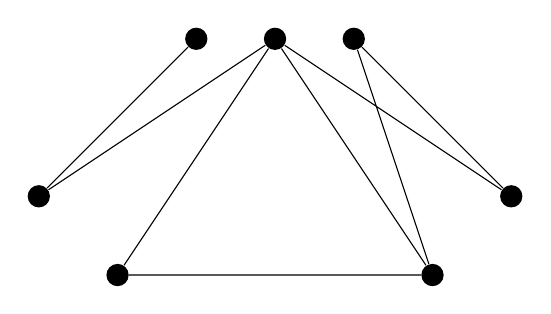
\begin{tikzpicture}[every node/.style = {circle, fill=black, inner sep=1mm}]
    \node (a1) at (-3, 1) {} % left, top
    node (a2) at (-2, 0) {} % left, bottom
    node (b1) at (-1, 3) {} % top, left
    node (b2) at (0, 3) {} % top, middle
    node (b3) at (1, 3) {} % top, right
    node (c1) at (2, 0) {} % right, bottom
    node (c2) at (3, 1) {}; % right, top
    \draw (b1) -- (a1) -- (b2) -- (a2) -- (c1) -- (b2) -- (c2) -- (b3) -- (c1);
  \end{tikzpicture}
}%

This section is the chapter one in the textbook "Introduction to Graph Theory". It covers all key concepts, keywords, definitions, theorems, etc.

\subsection{Graph}

\begin{definition}{}{con-graph}
  (1.1.2. Definition in text, modified version)
  A \textbf{graph} $G$ contains:
  \begin{enumerate}
    \item A \textbf{vertex set} $V(G)$
    \item An \textbf{edge set} $E(G)$
    \item A relation that associates with each two vertices (not necessarily distinct) called its \textbf{endpoints}.
  \end{enumerate}
\end{definition}

\Cref{def:con-graph} is a \textit{triple}, which means you need these three components to describe a graph, usually in the order of vertex set, edge set, and relations.

In \cref{def:con-graph}, for simple graphs, you could use a vertex set with either \textit{an edge set} or \textit{a relation for each edge} to define a graph. But for multigraphs like \cref{fig:con-graph}, in which there are multiple edges (\cref{def:con-loop}) between some two vertices, all three components of a graph are nontrivial.

An edge between vertices $u$ and $v$ can be denoted by either $\set{ u,\, v }$, $uv$ or $\left( u,\, v \right)$.

In \cref{def:con-graph}, the relation of a graph may$\ldots$
\begin{enumerate*}
  \item show the endpoints of \textit{each} edge in its edge set, or
  \item \textit{group} edges with the same endpoints and show the number of each group.
\end{enumerate*}

\begin{figure}[ht]
  \centering
  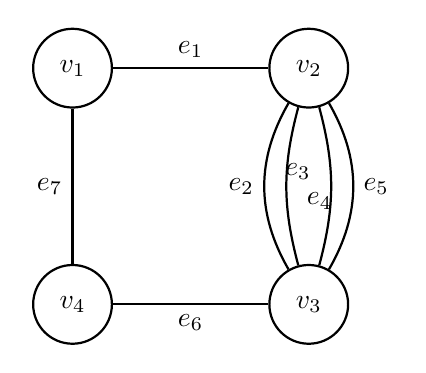
\begin{tikzpicture}[thick,
      main/.style = {draw, circle, minimum size=10mm},
      auto]
    % nodes
    \node[main] (1) at (0, 3) {$v_1$};
    \node[main] (2) at (3, 3) {$v_2$};
    \node[main] (3) at (3, 0) {$v_3$};
    \node[main] (4) at (0, 0) {$v_4$};

    % directed edges
    \draw (1) to node[above] {$e_1$} (2);
    \draw (2) to[bend right=30] node[left] {$e_2$} (3);
    \draw (2) to[bend right=15] node[right=-1.5mm, pos=.4] {$e_3$} (3);
    \draw (2) to[bend left=15] node[left=-1.5mm, pos=.6] {$e_4$} (3);
    \draw (2) to[bend left=30] node[right] {$e_5$} (3);
    \draw (3) to node[below] {$e_6$} (4);
    \draw (4) to node[left] {$e_7$} (1);
  \end{tikzpicture}
  \caption{A sample multigraph (opposite to a simple graph)}
  \label{fig:con-graph}
\end{figure}

\subsubsection{Seven Bridges of Königsberg}\label{subsubsec:con-seven-bridges}

Graph theory has been booming since 17th to 19th centuries.\footnote{In 1736, Leonhard Euler published a paper related to the Seven Bridges of Königsberg. This paper is regarded as the first paper in the history of graph theory, collected in \textit{Graph Theory, 1736--1936}, first published in 1976.} The initiation is the seven bridges problem in Prussia (now Russia).

In this problem, there are seven bridges among two mainlands and two islands on the Pregel river. The goal is to find a path to traverse all bridges exactly once and back to the starting point. See \cref{subsec:con-path} for more info about a path.

We have a graph as follows, shown in \cref{fig:con-seven-bridge}.
% ref: https://stackoverflow.com/a/33801400
\begin{equation*}
  G =
  \left(
  \begin{array}{l}
    \{ w,\, x,\, y,\, z \},                        \\
    \{ \foreach \i in {1,...,6} {e_\i,\, } e_7 \}, \\
    \{ wx,\, wx,\, wz,\, wz,\, wy,\, xy,\, yz \}
  \end{array}
  \right)
\end{equation*}

\begin{figure}[ht]
  \centering
  \begin{subfigure}{0.35\textwidth}
    \centering
    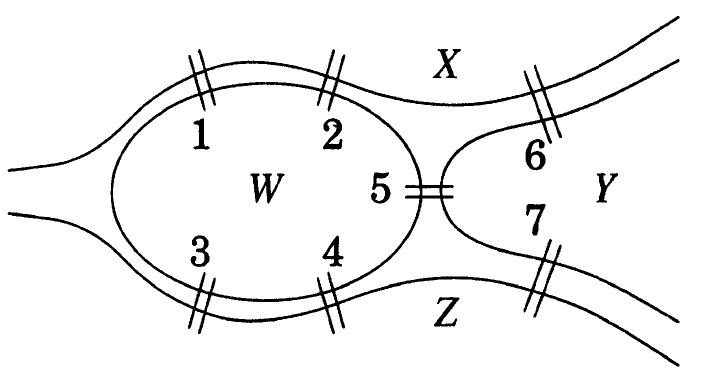
\includegraphics[width=\textwidth]{con-seven-bridge-original}
    \caption{Original version.}
    \label{fig:con-seven-bridge-original}
  \end{subfigure}
  \hspace{.1\textwidth}
  \begin{subfigure}{0.25\textwidth}
    \centering
    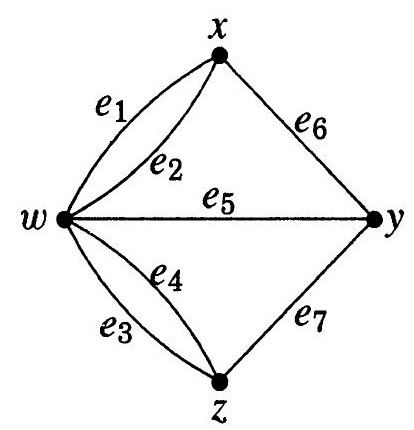
\includegraphics[width=\textwidth]{con-seven-bridge-graph}
    \caption{Graph version.}
    \label{fig:con-seven-bridge-graph}
  \end{subfigure}
  \caption{Seven-bridge problem.}
  \label{fig:con-seven-bridge}
\end{figure}

There are three principles related to the seven-bridge problem. You could try to list them on your own in advance:
\begin{enumerate*}
  \item If the degree (the number of connected edges) of each vertex is \textbf{even}, there must be a path to traverse all edges exactly once from and to the same vertex for an arbitrary vertex.
  \item If there are exactly \textbf{two} odd-degreed vertices, saying A and B, there must be a path to traverse all edges exactly once from A to B, or from B to A.
  \item If there are more than two odd-degreed vertices, three is no path to traverse all edges exactly once.
\end{enumerate*}

In the exams, you need to show why some graphs have no feasible solution with these three principles rather than showing all possible solutions.

We will cover the proofs of these principles in later sections. % TODO: link to their proofs

\subsubsection{Graph Terminologies}

\begin{definition}{}{con-loop}
  (1.1.4. Definition in text)
  A \textbf{loop} (so-called \textbf{self-loop}) is an edge whose endpoints are equal.

  \textbf{Multiple edges} are edges having the same pair of endpoints, like edges between $v_2$ and $v_3$ in a multigraph like \cref{fig:con-graph}.

  A \textbf{simple graph} is a graph having no loops or multiple edges.

  When $u$ and $v$ are the endpoints of an edge, they are \textbf{adjacent} and are \textbf{neighbors}, written $u \leftrightarrow v$.
\end{definition}

Continuing from \cref{def:con-loop}, if we have a node without a visible edge from an to it on graph, we wouldn't say that there is a self-loop.

\begin{definition}{}{con-finite-null-graph}
  (1.1.6.* Remark and the paragraph above it in text\footnote{The asterisk symbol (*) in the textbook \textit{Introduction to Graph Theory} means optional material that is not used later and can be skipped.})
  A \textbf{finite graph} has finite vertex set and edge set.

  A \textbf{null graph} (order-zero graph) has empty vertex set, and thus has empty edge set. Sometimes a null graph refers to an empty graph.

  An \textbf{empty graph} (edgeless graph) has finite vertex set and \textbf{empty} edge set.

  As for an \textbf{infinite graph}, it is usually used in Astronomy for infinite number of planets.
\end{definition}

Notice that in most cases, unless specified, we treat a graph as a simple and finite graph. In some cases, we consider null graphs and multigraphs.

\begin{definition}{}{con-complement}
  (1.1.8. Definition in text)
  The \textbf{complement} of a \textit{simple} graph $G$ is denoted by $\bar G$, which is the simple graph with vertex set $V(G)$ and edge set $E(\bar G)$ defined by $uv \in E(\bar G) \iff uv \notin E(G)$.

  A \textbf{clique} in a graph is a set of pairwise adjacent vertices. A single vertex is also a clique. However, it is controversial for a null graph to be a clique.

  An \textbf{independent set} (stable set) in a graph is a set of pairwise nonadjacent vertices.
\end{definition}

\begin{figure}[ht]
  \centering
  \begin{subfigure}[t]{.3\textwidth}
    \centering
    % TODO: TikZ version
    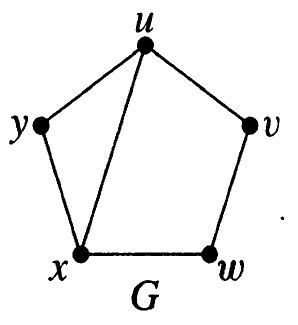
\includegraphics[width=\textwidth]{con-complement-before}
    \caption{The original graph $G$.}
    \label{fig:con-complement-before}
  \end{subfigure}
  \hspace{.1\textwidth}
  \begin{subfigure}[t]{.3\textwidth}
    \centering
    % TODO: TikZ version
    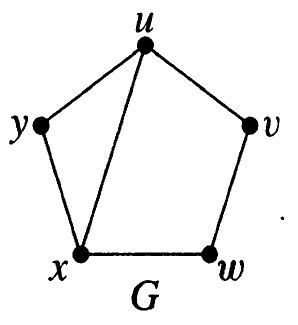
\includegraphics[width=\textwidth]{con-complement-before}
    \caption{The complement of graph $G$, denoted by $\bar G$.}
    \label{fig:con-complement-after}
  \end{subfigure}
  \caption{An example of complement of a graph. Also, vertices $u$, $x$ and $y$ in graph $G$ form a \textbf{maximal clique} of size 3 (three vertices); vertices $x$ and $w$ form a clique of size 2; vertex $u$ form a clique of size 1.}
  \label{fig:con-complement}
\end{figure}

For the complement in \cref{def:con-complement}, in brief, a complement of a graph $G$ consists of the same vertices of $G$ with all the edges \textit{not} in $G$ and without all the edges in $G$.

For the clique in \cref{def:con-complement}, note that a clique refers to a subset of vertices rather than edges or graphs.

When saying about a clique or an independent set, we usually need to find a maximal clique or a maximal independent set.

Finding a maximal clique and finding a maximal independent set are dual of each other. That is, finding a maximal clique in a graph $G$ (vertices $u,\, x,\, y$ in \cref{fig:con-complement-before}) is equal to finding an independent set in $\bar G$ (vertices $u,\, x,\, y$ in \cref{fig:con-complement-after}). \supp{If we find a maximal clique $C$ in $G$, since all vertices in $C$ are adjacent, they are all nonadjacent in $\bar G$, and it means a maximal independent set in $\bar G$.}

Finding a maximal clique, finding all cliques and finding a maximal independent set are all NP-complete problems.
And finding a maximal independent set is also a strongly NP-hard problem.

\begin{definition}{}{con-chromatic}
  (1.1.12. Definition in text)
  \textbf{Chromatic number} of a graph $G$, denoted by $\chi (G)$, is the \textit{minimum number of colors} needed to label the vertices so that adjacent vertices receive different colors.
\end{definition}

For \cref{def:con-chromatic}, that is, if two vertices has an edge between, these two vertices cannot have the same color. For a tree (because it's bipartite as shown in \cref{prop:con-bipartite-tree}), its chromatic number is 2. For a graph without edges, its chromatic number is 1.

For any finite graph (\cref{def:con-finite-null-graph}), we can find its chromatic number given that the colors can be hard for humans to distinguish (like \#FF1234 and \#FF1235 pixel values).

\supp{Chromatic numbers The complexity of finding a chromatic number is an open problem. It is likely NP-complete or NP-hard, but we couldn't find a way to reduce it to an NP-complete problem.}

\subsubsection{Bipartite Graphs}

\begin{recallable}{definition}{}{con-bipartite}
  (1.1.10. Definition and 1.1.12. Definition in text)
  A graph $G$ is \textbf{bipartite} if $V(G)$ is the union of two disjoint (possibly empty) \textit{independent sets} called \textbf{bipartite sets} of $G$.

  For three disjoint independent sets, $G$ is \textbf{tripartite}.

  For $k$ disjoint independent sets, $G$ is $k$-partite (generally speaking, multipartite), where $k \in \set{ i : i \in \N \land i \geq 3}$.
\end{recallable}

\begin{figure*}[ht]
  \centering
  \begin{subfigure}{.4\textwidth}
    \centering
    \bipartitegraphwithlabels
    \caption{A bipartite graph}
    \label{fig:con-bipartite}
  \end{subfigure}
  \hspace{.1\textwidth}
  \begin{subfigure}{.4\textwidth}
    \centering
    \tripartitegraph
    \caption{A tripartite graph.}
    \label{fig:con-tripartite}
  \end{subfigure}
  \caption{Bipartite and tripartite graphs.}
  \label{fig:con-bipartite-tripartite}
\end{figure*}

In \cref{fig:con-bipartite}, only people can get paid for jobs; people cannot get people (having no relation); jobs cannot get jobs. Thus, the following graph is a \textbf{bipartite graph}.

However, it is possible for all the people here to get no offers (jobs). This is a special case you need to consider in exams.

In a rooted tree like \cref{fig:con-rooted-tree}, you are able to see the children and parents of nodes, so you can find a root. In an unrooted tree like \cref{fig:con-unrooted-tree}, you couldn't. % TODO: link to tree

\begin{figure}[ht]
  \centering
  \begin{subfigure}[t]{.2\textwidth}
    \centering
    % TODO: TikZ version
    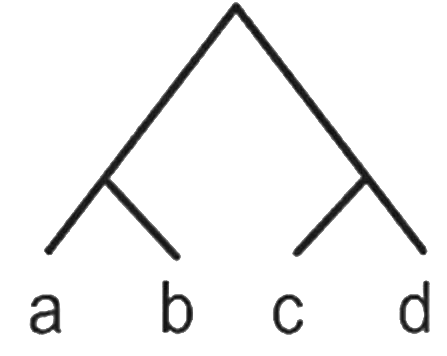
\includegraphics[width=\textwidth]{con-rooted-tree}
    \caption{A rooted tree}
    \label{fig:con-rooted-tree}
  \end{subfigure}
  \hspace{.1\textwidth}
  \begin{subfigure}[t]{.2\textwidth}
    \centering
    % TODO: TikZ version
    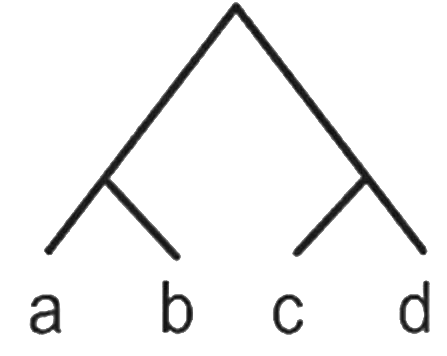
\includegraphics[width=.8\textwidth]{con-unrooted-tree}
    \caption{An unrooted tree}
    \label{fig:con-unrooted-tree}
  \end{subfigure}
  \hspace{.1\textwidth}
  \begin{subfigure}[t]{.3\textwidth}
    \centering
    % TODO: TikZ version
    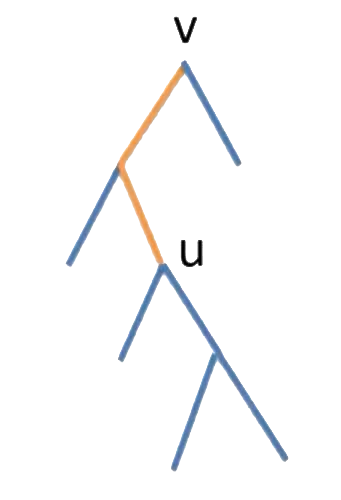
\includegraphics[width=.5\textwidth]{con-bipartite-tree}
    \caption{An illustration to prove that a rooted tree is a bipartite graph}
    \label{fig:con-bipartite-tree}
  \end{subfigure}
  \caption{Examples of rooted trees and unrooted trees}
  \label{fig:con-rooted-unrooted-trees}
\end{figure}

In programming, you could use linked lists to store a tree, but in graph theory, rooted and unrooted trees have different meaning.

\begin{proposition}{}{con-bipartite-tree}
  A tree (either rooted or unrooted one) is bipartite.
\end{proposition}

\textbf{Proof} of \cref{prop:con-bipartite-tree}:
Our goal is to find a partition of two disjoint independent sets.
Let $v$ be the root of a tree (we could pick any node, but this node is fixed in the following proof), and let $u$ be an arbitrary node in the tree.
We can find the distance between $v$ and $u$, and such a distance is a non-negative integer ($\N \cap \{ 0 \}$).
We partition all nodes in the tree into two sets: a set $S_e$ for all nodes with even distances to $v$, including $v$ itself; a set $S_o$ for all nodes with odd distances to $v$.
There is no exception for non-even and non-odd distances.
Since $S_e$ and $S_o$ are disjoint independent sets, the tree is a bipartite graph.
This applies to all trees including rooted and unrooted trees.

So, for a coloring problem on a tree, we could apply the same technique above to find two independent sets to solve the problem. We could also prove \cref{prop:con-bipartite-tree} with a coloring problem. % TODO: link to coloring problem

Note that some proofs are pretty simple, but it doesn't mean that they wouldn't be in exams.

Some comments for bipartite graphs:
\begin{enumerate}
  \item \label{enum:con-bipartite-odd} A bipartite graph is a graph with no odd length cycle. That is, there doesn't exist a path to traverse some vertices along edges and back to the starting point with odd number of edges. For a graph with no possible cycles or with only even length cycles, such a graph is also bipartite. \supp{A bonus problem is as follows. Proove that a graph is not bipartite if it has one or more \textit{arbitrary} (3, 5, 7, etc.) odd length cycles. However, in 2024 spring, announced in 2024-03-08, the bonus problem changed to a program homework with different topics.}

  \item Another ways to define an $n$-vertex tree $G$, where $n \geq 1$:
        \begin{enumerate}
          \item $G$ satisfies any two of the following three rules:
                \begin{enumerate}
                  \item $G$ is connected. (See \cref{fig:con-connected-graph-interlude} for the illustration of connected and unconnected graphs. And see \cref{def:con-connected} for the definition.)
                  \item $G$ has "$n - 1$" edges.
                  \item $G$ has no cycles. Note that a self-loop is a cycle.
                \end{enumerate}
          \item $G$ has no loops, and for each $u,\, v \in V(G)$, there exists exactly one $u,\, v$-path. (This rule is sufficient to show that $G$ is a tree, for the later part shows the three rules above.) % TODO: link to their proofs
        \end{enumerate}
\end{enumerate}

Note that a graph $G$ with "$n - 1$" edges doesn't mean $G$ is connected. For example, a graph with two components: one is a triangle with three vertices and three edges, and the other one is an isolated graph with a vertex. Such a graph is 4 vertices with 3 edges, but is disconnected.

\supp{In the above-mentioned definition of a tree, we could pick two rules in three because in their proofs, they show that any two satisfied rules imply the other rule in a circular way.}

\begin{figure}[ht]
  \centering
  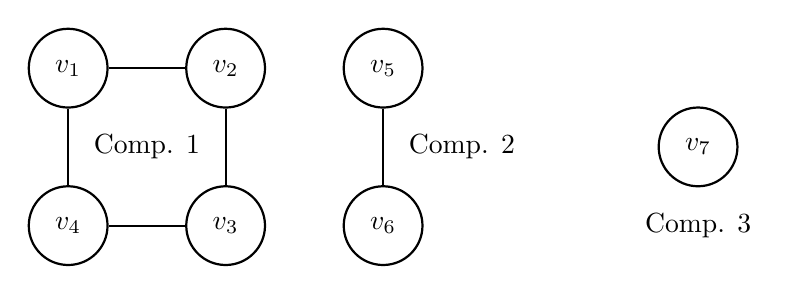
\begin{tikzpicture}[thick,
      main/.style = {draw, circle, minimum size=10mm},
      auto]
    % nodes
    \node[main] (1) at (0, 2) {$v_1$};
    \node[main] (2) at (2, 2) {$v_2$};
    \node[main] (3) at (2, 0) {$v_3$};
    \node[main] (4) at (0, 0) {$v_4$};
    \node at (1, 1) {Comp. 1};

    \node[main] (5) at (4, 2) {$v_5$};
    \node[main] (6) at (4, 0) {$v_6$};
    \node at (5, 1) {Comp. 2};

    \node[main] (7) at (8, 1) {$v_7$};
    \node at (8, 0) {Comp. 3};

    % undirected edges
    \draw (1) -- (2) -- (3) -- (4) -- (1);
    \draw (5) -- (6);

  \end{tikzpicture}
  \caption{An unconnected graph with three sub-components (connected subgraph). If we removes vertices $v_5$, $v_6$ and $v_7$, we would have a connected graph with exactly one component. In brief, in a connected graph, each two nodes $u,\, v$ has at least one path. See \cref{def:con-connected} for the definition of connected and unconnected graphs.}
  \label{fig:con-connected-graph-interlude}
\end{figure}

\subsection{Paths, Cycles and Trails}\label{subsec:con-path}

\begin{definition}{}{con-path-cycle}
  (1.1.15. Definition in text)
  A \textbf{path} is a (ordered) \textbf{sequence} of \textit{distinct} vertices such that any two consecutive vertices are adjacent. We call $v_0$ and $v_k$ the endpoints of the path $\anglebrackets{v_0,\, v_1,\, \ldots,\, v_k}$.

  A \textbf{cycle} is a sequence of vertices, where all vertices except the last vertex are distinct, and the two endpoints are equal, such that any two consecutive vertices are adjacent. For example, $\anglebrackets{v_0,\, v_1,\, \ldots,\, v_k,\, v_0}$.
\end{definition}

In \cref{def:con-path-cycle}, note that a path or a cycle refers to a set of vertices instead of edges, although any two consecutive vertices being adjacent implies edges.

There are examples for \cref{def:con-path-cycle} in \cref{fig:con-path-cycle}. Note that in \cref{fig:con-cycle}, the intersection point of edges $xb$ and $yz$ is not a vertex.

In \cref{fig:con-path}, reversing the order of vertices in the given path gives another path by definition. The vertex sequence matters. Same for \cref{fig:con-cycle}; starting from $a$ back to $a$ and starting from $b$ back to $b$ yield two different cycles, and if you go in the other direction, you have another two different cycles in definition.

\begin{figure}[ht]
  \def \nodelist {
    \node[main] (x) at (0, 1.5) {$x$}
    node[main] (y) at (0, 0) {$y$}
    node[main] (z) at (1.5, 1.5) {$z$}
    node[main] (b) at (1.5, 0) {$b$}
    node[main] (a) at (3, 0.75) {$a$};}

  \centering
  \begin{subfigure}{.3\textwidth}
    \centering
    \begin{tikzpicture}[
        main/.style = {draw, circle}
      ]
      \nodelist
      \draw (x) -- (b) -- (a) -- (z) -- (y);
    \end{tikzpicture}
    \caption{$\anglebrackets{x,\, b,\, a,\, z,\, y}$ is a path.}
    \label{fig:con-path}
  \end{subfigure}
  \begin{subfigure}{.3\textwidth}
    \centering
    \begin{tikzpicture}[
        main/.style = {draw, circle}
      ]
      \nodelist
      \draw (x) -- (b) -- (a) -- (z) -- (y) -- (x);
    \end{tikzpicture}
    \caption{$\anglebrackets{a,\, b,\, x,\, y,\, z,\, a}$ is a cycle.}
    \label{fig:con-cycle}
  \end{subfigure}

  \caption{Examples for a path and a cycle for \cref{def:con-path-cycle}.}
  \label{fig:con-path-cycle}
\end{figure}

\begin{definition}{}{con-subgraph}
  (1.1.16. Definition in text)
  A \textbf{subgraph} of $G$ is a graph $S$ such that $\ldots$
  \begin{enumerate*}
    \item $V(S) \subseteq V(G)$ and
    \item $E(S) \subseteq E(G)$ and
    \item the assignment of endpoints to edges in $S$ is the same in $G$.
  \end{enumerate*}

  The third requirement means that for vertices $u$ and $v$ in $S$, there won't be an edge $uv$ if there is no such an edge in $G$.

  We denote $S \subseteq G$ for a subgraph of a graph $G$.
\end{definition}

For \cref{def:con-subgraph}, in other words, if $S \subseteq G$, all vertices and edges in $S$ are in $G$ without introducing new vertices or edges. Later, we will cover induced subgraphs, which pose a constraint on edges. % TODO: link to induced subgraphs

\begin{definition}{Connected graphs}{con-connected}
  (1.1.16. Definition in text)
  A graph $G$ is \textbf{connected} if each pair of vertices in $G$ belongs to a path. Otherwise, $G$ is \textbf{disconnected}.
\end{definition}

For \cref{def:con-connected}, in other words, if a graph $G$ is connected, you can find a path from any one vertex to each other vertices. % TODO: link to its definition with components

See \cref{fig:con-connected-unconnected} for the examples of \cref{def:con-connected}.

\begin{figure}[ht]
  % ref using inner sep to set maximum size: https://tex.stackexchange.com/a/228365
  % ref for every node: https://tex.stackexchange.com/a/78718
  \centering
  \begin{subfigure}[t]{.4\textwidth}
    \centering
    \tripartitegraph
    \caption{A connected graph.}
    \label{fig:con-connected}
  \end{subfigure}
  \begin{subfigure}[t]{.4\textwidth}
    \centering
    \bipartitegraph
    \caption{An unconnected graph (with two connected subgraphs) even though it is bipartite (\cref{def:con-bipartite}).}
    \label{fig:con-unconnected}
  \end{subfigure}
  \caption{Examples for a connected graph and an unconnected graph.}
  \label{fig:con-connected-unconnected}
\end{figure}

\subsection{Graph Isomorphism}\label{subsec:con-graph-isomorphism}

\begin{definition}{}{con-adj}
  (1.1.17. Definition in text)
  Let $G$ be a loopless graph with vertex set $V(G) = \set{ v_1,\, v_2,\, \ldots,\, v_n}$ and edge set $E(G) = \set{ e_1,\, e_2,\, \ldots,\, e_m}$:

  \begin{enumerate}
    \item The \textbf{adjacency matrix} of $G$, written $A(G)$, is an $n$-by-$n$ matrix where entry $a_{i,j}$ is the number of edges in $G$ with endpoints $\set{v_i,\, v_j}$.
    \item The \textbf{incidence matrix} of $G$, written $M(G)$, is an $n$-by-$m$ matrix where entry $m_{i,j}$ is 1 if $v_i$ is an endpoint of edge $e_j$. Otherwise, $m_{i,j}$ is 0.
  \end{enumerate}

  A vertex $v$ is \textbf{incident} with an edge $e$ if $v$ is an endpoint of $e$. (cf. \textit{adjacent} in \cref{def:con-loop}: $u$ and $v$ are adjacent/neighbors if $u$ and $v$ are the endpoints of an edge $e$.)

  The \textbf{degree} of a vertex $v$ in a loopless undirected graph is the number of incident (incoming) edges of $v$. In an undirected graph, an edge is both incoming and outgoing to both its endpoints.

  In a directed graph, the \textbf{indegree} of a vertex $v$ is the number of incoming edges (arrows); the \textbf{outdegree} of a vertex $v$ is the number of outgoing edges (tails).
\end{definition}

In \cref{def:con-adj}, in brief, the adjacency matrix records the number of edges between each two vertices; the incidence matrix records the endpoints of each edge. See \cref{fig:con-adj} for some examples.

(1.1.18 Remark) The adjacency matrix of a simple graph consists of 0 and/or 1. In a simple undirected graph, the adjacency matrix is always \textbf{symmetric} ($A(G) = A(G)^\trans$) with all zeros on the diagonal.

In a finite graph, the incidence matrix consists of 0 and/or 1, and each vertex has a degree (at least 0).

\begin{figure}[ht]
  \centering
  % TODO: TikZ and blkarray versions
  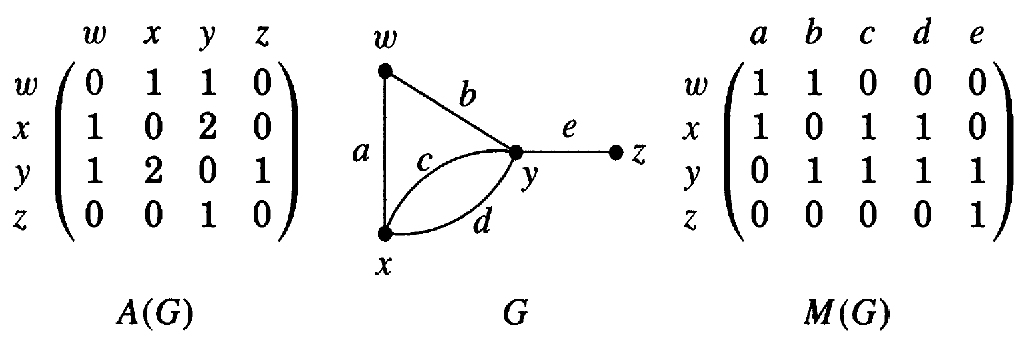
\includegraphics[width=.8\textwidth]{con-adj}
  \caption{A graph $G$ with its adjacency matrix $A(G)$ and incidence matrix $M(G)$. $a_{i,j}$ in $A(G)$ is $\set{v_i,\, v_j}$ in $G$.}
  \label{fig:con-adj}
\end{figure}

\begin{definition}{}{con-isomorphism}
  (1.1.20. Definition in text)
  An \textbf{isomorphism} from a \textbf{simple graph} $G$ to a \textbf{simple graph} $H$ is a \textbf{bijection function} (equivalent relation; \cref{def:intro-equiv-relation}) $\func{f}{V(G)}{V(H)}$ such that $uv \in E(G) \iff f(u)f(v) \in E(H)$. See \cref{def:con-loop} for the definition of simple graphs.

  We say "$G$ is \textbf{isomorphic to} $H$", written $G \isomorphicto H$, if there is an isomorphism from $G$ to $H$.
\end{definition}

You could recall three special function, including a bijective function as shown in \cref{fig:intro-special-functions}.
\reusefigure[ht]{fig:intro-special-functions}

For \cref{def:con-isomorphism}, in other words, a graph $G$ is isomorphic to a graph $H$ if and only if there exists a bijection function $\func{f}{V(G)}{V(H)}$, where $V(G)$ and $V(H)$ are vertices sets of $G$ and $H$ respectively, such that for every edge $uv$ in $G$, there is a corresponding edge $f(u)f(v)$ in $H$, and vice versa, without introducing additional vertices or edges.

For two isomorphic graphs $G$ and $H$, they may look different by human eyes. And note that a prerequisite for isomorphism is the same number of vertices and the same number of degrees. With different numbers of vertices or a degree that is absent one graph, the two graphs cannot be isomorphic. But with the same number of vertices and the same number of degrees, we still need a bijection function to prove the isomorphism from one graph to the other one.

See \cref{fig:con-isomorphism} for an example. In this example, we could see that vertices $w,\, z$ may correspond to $c,\, a$; and $x,\, y$ to $b,\, d$.

\begin{figure}[ht]
  \centering
  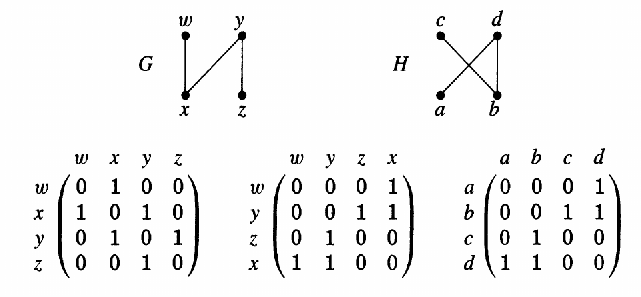
\includegraphics[width=.7\textwidth]{con-isomorphism}
  \caption{An example that $G$ is isomorphic to $H$. The following three matrices are adjacency matrices.}
  \label{fig:con-isomorphism}
\end{figure}

\supp{
  In programming, to determine whether graphs $G$ and $H$ are isomorphic to each other, we could build adjacency matrices for these two graphs (matrices 1 and 3 in \cref{fig:con-isomorphism}) respectively after fixing the order of vertices in $H$ to $a,\, b,\, c,\, d$ and choosing an order of vertices in $G$. Later, if the two adjacency matrices are different, change the order of vertices in $G$ to the other untested order, saying $w,\, y,\, z,\, x$, and then build the adjacency matrix of $G$ according to the new order. Note that for a new order of vertices, you cannot simply swap columns in the matrix because the row order changes as well. Once the adjacency matrices of $G$ and $H$ are identical like the matrices 2 and 2 in \cref{fig:con-isomorphism}, we could find the bijection function for vertex sets of $G$ and $H$. In \cref{fig:con-isomorphism}, vertices $w,\, y,\, z,\, x$ in $G$ correspond to vertices $a,\, b,\, c,\, d$ in $H$ respectively.

  The complexity of graph isomorphism is an open problem. It is highly possible not a $P$ problem. By the say, the subgraph problem (determining whether a smaller graph is isomorphic to some subgraph(s) in a larger graph) is NP-complete.

  A bonus problem (not in 2024 spring) is as follows. How do you define two multigraphs (including the cases of multiple edges and loops; see \cref{def:con-loop} for definition) are isomorphism? We need definition rather than proofs. Isomorphism in multigraphs is possible in real world. There is no commonly approved definition, but many different definitions you can reference. Note that graph (multigraph) isomorphism always follows the principle of bijection (one-to-one correspondence). Your answer has to be handwritten in Chinese clearly, possibly using the same ideas from references.
}

Recall \cref{def:intro-equiv-relation} as follows.
\recall[\sectionprefix]{intro-equiv-relation}

\supp{Friendship relation is not always an equivalence relation. Relation in law is an equivalence relation. An equivalence relation in graph theory is commonly used to collect all sets with the same relation.}

\begin{proposition}{}{con-iso-equiv}
  (1.1.24. Proposition in text)
  The isomorphism relation is an equivalence relation on the set of \textbf{simple} graphs.
\end{proposition}

\textbf{Proof} of \cref{prop:con-iso-equiv}:

\begin{enumerate}
  \item Reflexive: $G \isomorphicto G$. (A graph and itself have isomorphism relation.)
  \item Symmetric: $uv \in E(G) \iff f(u)f(v) \in E(H)$ yields $xy \in E(H) \iff f^{-1}(x)f^{-1}(y) \in E(G)$. So, $G \isomorphicto H \iff H \isomorphicto G$. Consider $f$ and its inverse ($f^{-1}$) to be bijection functions.
  \item Transitive:
        \begin{enumerate}
          \item See \cref{fig:con-iso-equiv} for the illustration.
          \item Let $\func{f}{V(F)}{V(G)}$ and $\func{g}{V(G)}{V(H)}$ be two isomorphism relation functions.
          \item Given $uv \in E(F) \iff f(u)f(v) \in E(G)$ and $xy \in E(G) \iff g(x)g(y) \in E(H)$ by definition, since $f$ is an isomorphism, for every $xy \in E(G)$ we can find $uv \in E(G)$ such that $f(u) = x$ and $f(v) = y$.
          \item The last statement yields $uv \in E(F) \iff g(f(u))g(f(v)) \in E(H)$, where $f(u) = x$ and $f(v) = y$.
          \item Thus, the composition $g \composition f$ is an isomorphism from $F$ to $H$.
          \item We have proved that $F \isomorphicto G$ and $G \isomorphicto H$ together imply $F \isomorphicto H$.
        \end{enumerate}
\end{enumerate}

\begin{figure}[htbp]
  \def\hoffset{3cm}%
  \def\voffset{1.2cm}%
  \def\domain#1#2{\draw[fill=#2] (\hoffset * #1, 0) ellipse (1cm and 2cm)}%
  \def\elements#1#2#3#4{
    \node[main] (#3) at (\hoffset * #1, \voffset) {$#3$}
    node[main] (#4) at (\hoffset * #1, 0) {$#4$}
    node at (\hoffset * #1, -\voffset) {$#2$};
    \draw[edge] (#3) -- (#4)
  }
  \centering
  \begin{tikzpicture}[
      main/.style = {draw, circle, fill=white, minimum size=.8cm},
      edge/.style = {thick},
      trans/.style = {dashed, -Latex}
    ]
    \foreach \d/\c in {1/yellow, 2/green, 3/cyan}
    \domain{\d}{\c};

    \foreach \i/\d/\a/\b in {1/F/u/v, 2/G/x/y, 3/H/a/b}
    \elements{\i}{\d}{\a}{\b};

    \foreach \a/\f/\x in {u/f/x, v/f/y, x/g/a, y/g/b}
    \draw[trans] (\a) to node[midway, above] {$\f$} (\x);
  \end{tikzpicture}
  \caption{An illustration for the transitive property of isomorphism in \cref{prop:con-iso-equiv}. Given $F \isomorphicto G$ by a function $f$ and $G \isomorphicto H$ by a function $g$, $f \composition g$ is also a bijection function and an isomorphism.}
  \label{fig:con-iso-equiv}
\end{figure}

If we have some graphs isomorphic to one another; that is, satisfying the proofs of \cref{prop:con-iso-equiv} for each one, each two, each three of graphs, we could use a set to collect all of such graphs. Such a set is an \textbf{equivalence class} (\textbf{equivalence set}). \supp{A star and a pentagon are in the same equivalence class.}

\begin{definition}{}{con-complete}
  (1.1.27. Definition in text)
  A \textbf{complete graph} $K_n$ is a simple graph whose vertices are \textbf{pairwise} adjacent; $K_n$ denotes the \textbf{unlabeled} complete graph with $n$ vertices.

  A \textbf{complete bipartite graph} $K_{r,s}$ or \textbf{biclique} is a simple bipartite graph such that two vertices are adjacent iff. they are in different partite sets.
\end{definition}

For \cref{def:con-complete}, a complete graph with $n$ vertices is $K_n$ rather than $C_n$, which refers to a cycle. $P_n$ is a path. You couldn't rename them, for they are well-known in graph theory.

A complete bipartite graph is not a complete graph. Nonetheless, $K_{r,s}$ is a subgraph of $K_n$, given $r \leq n$ and $s \leq n$.

$C_3$ is a subgraph of $K_5$. In a $K_5$, there are $C_5^3 = 10$ (combination) distinct $C_3$. However, in $K_{2,3}$, there is no $C_3$, which is an odd-length cycle. See Theorem 1.2.18, comment \ref{enum:con-bipartite-odd} in \cpageref{enum:con-bipartite-odd} and \cref{rem:intro-equal-sets} in \cpageref{rem:intro-equal-sets} for the definition of bipartite graphs. % TODO: link to Theorem 1.2.18

\begin{figure}[htbp]
  \centering
  \begin{subfigure}[t]{.4\textwidth}
    \centering
    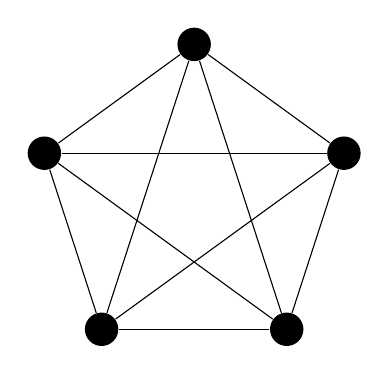
\begin{tikzpicture}[every node/.style = {circle, fill=black, inner sep=1.5mm}]
      \def\num{5}%
      \def\degoffset{360 / \num}%
      \foreach \i in {1,...,\num}{
          \node (\i) at (\degoffset * \i + 90 : 2) {};
          \foreach \j in {1,...,\i}{
              \ifthenelse{\i = \j}{}{
                \draw (\i) -- (\j);
              }
            }
        }
    \end{tikzpicture}
    \caption{$K_5$: A complete graph with 5 vertices.}
    \label{fig:con-complete}
  \end{subfigure}
  \hspace{2cm}
  \begin{subfigure}[t]{.4\textwidth}
    \centering
    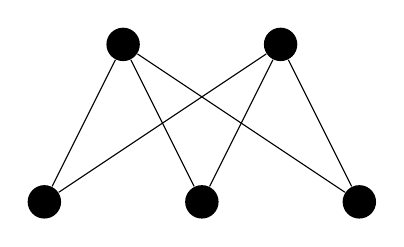
\begin{tikzpicture}[every node/.style = {circle, fill=black, inner sep=1.5mm}]
      \def\numi{2}%
      \def\numj{3}%
      \node foreach \i in {1,...,\numi} (a\i) at (2 * \i - 2, +1) {};
      \node foreach \j in {1,...,\numj} (b\j) at (2 * \j - 3, -1) {};

      \foreach \i in {1,...,\numi}
      \foreach \j in {1,...,\numj}
      \draw (a\i) -- (b\j);
    \end{tikzpicture}
    \caption{$K_{2,3}$: A complete bipartite graph with 2 and 3 vertices in partite sets respectively.}
    \label{fig:con-complete-bipartite}
  \end{subfigure}
  \caption{Examples for complete graphs and bipartite complete graphs.}
  \label{fig:con-complete-bipartite-full}
\end{figure}

\begin{example}{}{con-relation}
  (1.1.30. Example in text)
  Given the four figures as shown in \cref{fig:con-relation}, please answer the following questions.
  \begin{enumerate}
    \item \textbf{Question}: Which graphs are isomorphic to each other or one another?\\\textbf{Answer}: $G_1,\, G_2,\, G_4$ form an equivalence class. $G_3$ forms the other equivalence set.

    \item \textbf{Question}: Are the complement graphs of two isomorphic (simple) graphs also isomorphic?\\\textbf{Answer}: Yes.
  \end{enumerate}
\end{example}

\begin{figure}[htbp]
  % TODO: TikZ version
  \newcommand\quartersubfigure[4][width=.8\textwidth]{%
    \begin{subfigure}[t]{.2\textwidth}%
      \centering%
      \includegraphics[#1]{#2}%
      \caption{#3}%
      \label{#4}%
    \end{subfigure}%
  }%
  \centering
  \quartersubfigure[width=.6\textwidth]{con-relation-g1}{$G_1$ ($K_{3,3}$)}{fig:con-relation-g1}
  \quartersubfigure{con-relation-g2}{$G_2$ (hexagon)}{fig:con-relation-g2}
  \quartersubfigure{con-relation-g3}{$G_3$}{fig:con-relation-g3}
  \quartersubfigure{con-relation-g4}{$G_4$}{fig:con-relation-g4}
  \caption{Four figures for the relation examples.}
  \label{fig:con-relation}
\end{figure}

Detailed answer to question 1 in \cref{ex:con-relation}:
\begin{enumerate*}
  \item Suppose that $G_1$ and $G_2$ are an isomorphism.
  \item Select a fixed vertex mapping from $G_1$ to $G_2$, saying $u$ to 1.
  \item Since $u$ has three edges to vertices $x$, $y$, and $z$ respectively, in $G_2$, they such three vertices are mapped to 2, 4 and 6.
  \item After finding all one-to-one correspondences, you can show that $G_1$ is isomorphic to $G_2$.
  \item In the other way, since $G_1$ is $K_{3,3}$, if we find a way to convert $G_2$ to $K_{3,3}$, we can also show the isomorphism. For example, two disjoint and independent sets $\{ 1,\, 3,\, 5 \}$ and $\{ 2,\, 4,\, 6 \}$.
  \item In $G_3$, we can easily find two $C_3$ (as odd-length cycles), so $G_3$ is not bipartite; thus, cannot be isomorphic to $G_1$ or $G_2$. $C_3$ is isomorphic to $K_3$; $K_3$ is not a subgraph of $K_{3,3}$.
\end{enumerate*}

Detailed answer to question 2 in \cref{ex:con-relation}:
\begin{enumerate*}
  \item For vertices in a complement graph, they are identical to the original graph.
  \item By definition of a complement graph in \cref{def:con-complement}, the two complement graphs have the same relation. This required a proof, though.
  \item For example, the complement of $G_1$, $G_2$ or $G_4$ is a disconnected graph with two $C_3$ (triangle). The complement of $G_3$ is a $C_6$.
  \item In conclusion, you cannot know whether a complement graph is disconnected or connected given the original graph connected or disconnected.
  \item The complement of a \textbf{complete} bipartite graph with at least two vertices always has two components. Generally, the complement of a bipartite graph doesn't always a disconnected graph.
  \item You need to understand the logics thoroughly to pass exams.
\end{enumerate*}

\begin{definition}{}{con-self-comp}
  A graph is \textbf{self-complementary} if it is isomorphic to its complement.

  A \textbf{decomposition} of a graph is a list of subgraphs such that each edge appears in exactly one subgraph in ths list.

  An $n$-vertex graph $H$ is self-complementary \textbf{iff.} $K_n$ has a decomposition consisting of two copies of $H$. (Not proved in text)
\end{definition}

Consider only the thick edges in \cref{fig:con-self-comp-pentagon} as a graph; such a graph is self-complementary. However, $K_5$ is not self-complementary, for the complement of $G_5$ has no edges.

In exams, you may be asked whether $K_4$ can be decomposed by some copies of $P_3$ like \cref{fig:con-self-comp-rectangle}, where the numbers 4 and 3 may change. Note that each edge in the decomposition must appear exactly once. As shown in \cref{fig:con-self-comp-heptagon}, you could decompose $K_7$ with 7 copies of $C_3$. As shown in \cref{fig:con-self-comp-pentagon-cdot}, you could decompose $K_6$ with 6 copies of $P_4$.

You might have noticed that to decompose a graph $G$ by some copies of $H$, the number of edges in $G$ must be multiples of those in $H$. However, this is not sufficient to decompose $G$ in that way. For example, you couldn't decompose $K_5$ in \cref{fig:con-self-comp-pentagon} with two kites in \cref{fig:con-graph-menageries}.

\begin{figure}[htbp]
  \def \nodesize {.8mm}%
  \def \shapesize {1.5cm}%
  \def \subfiguresize {.4\textwidth}%
  \def \hseparation {.1\textwidth}%
  \centering
  \begin{subfigure}[t]{\subfiguresize}
    \centering
    \begin{tikzpicture}[every node/.style = {circle, fill=black, inner sep=\nodesize}]
      \def\num{5}%
      \def\degoffset{360 / \num}%
      % node 1 at topmost corner; count nodes clockwise
      % \degoffset * -(\i - 1) means clockwise offset degrees from node 1
      % + 90 to rotate left 90 degrees to make node 1 at top
      \node foreach \i in {1,...,\num} (\i) at (-\degoffset * \i + \degoffset + 90 : \shapesize) {};
      \foreach \i in {1,...,\num} {
          \draw[evaluate={\j=int(1+mod(\i, \num));}, ultra thick] (\i) -- (\j);
          \draw[evaluate={\j=int(1+mod(\i+1, \num));}] (\i) -- (\j);
        }
    \end{tikzpicture}
    \caption{A decomposition of $K_5$ could be two 5-cycles $C_5$, including the thick one and inner star. (1.1.33. Example in text)}
    \label{fig:con-self-comp-pentagon}
  \end{subfigure}
  \hspace{\hseparation}
  \begin{subfigure}[t]{\subfiguresize}
    \centering
    \begin{tikzpicture}[every node/.style = {circle, fill=black, inner sep=\nodesize}]
      \def\num{4}%
      \def\degoffset{360 / \num}%
      % node 1 at top-left corner; count nodes clockwise
      % \degoffset * -(\i - 1) means clockwise offset degrees from node 1
      % + 135 to rotate left 135 degrees to make node 1 at top-left corner
      \node foreach \i in {1,...,\num} (\i) at (-\degoffset * \i + \degoffset + 135 : \shapesize) {};
      \draw[ultra thick] (4) -- (1) -- (2);
      \draw (1) -- (3) -- (4);
      \draw[dashed] (3) -- (2) -- (4);
    \end{tikzpicture}
    \caption{A decompose of $K_4$ could be three $P_3$, including the thick, normal and dashed ones. (1.1.33. Example in text)}
    \label{fig:con-self-comp-rectangle}
  \end{subfigure}

  \vspace{1em}

  \begin{subfigure}[t]{\subfiguresize}
    \centering
    \begin{tikzpicture}[every node/.style = {circle, fill=black, inner sep=\nodesize}]
      \def\num{7}%
      \def\degoffset{360 / \num}%
      % node 1 at topmost corner; count nodes clockwise
      % \degoffset * -(\i - 1) means clockwise offset degrees from node 1
      % + 90 to rotate left 90 degrees to make node 1 at top
      \node foreach \i in {1,...,\num} (\i) at (-\degoffset * \i + \degoffset + 90 : \shapesize) {};
      \draw[ultra thick] (1) -- (2) -- (4) -- (1);
      \draw (2) -- (3) -- (5) -- (2);
      \draw[dashed] (3) -- (4) -- (6) -- (3);
    \end{tikzpicture}
    \caption{A decomposition of $K_7$ could be 7 triangles $C_3$ by rotating the thick one through seven possible positions like the normal and dashed ones. (1.1.34.* Example in text)}
    \label{fig:con-self-comp-heptagon}
  \end{subfigure}
  \hspace{\hseparation}
  \begin{subfigure}[t]{\subfiguresize}
    \centering
    \begin{tikzpicture}[every node/.style = {circle, fill=black, inner sep=\nodesize}]
      \def\num{5}%
      \def\degoffset{360 / \num}%
      % node 1 at top-left corner; count nodes clockwise
      % \degoffset * -(\i - 1) means clockwise offset degrees from node 1
      % + 90 to rotate left 90 degrees to make node 1 at top
      \node foreach \i in {1,...,\num} (\i) at (-\degoffset * \i + \degoffset + 90 : \shapesize) {};
      \node (6) {};
      \draw[ultra thick] (6) -- (1) -- (3) -- (2);
      \draw (6) -- (2) -- (4) -- (3);
    \end{tikzpicture}
    \caption{To decompose $K_6$, you could place a vertex at the center of a pentagon, and constructing a $P_4$ with edges from each of (1) the outer $C_5$, (2) the inner star $C_5$ and (3) the edges involving the center vertex. By rotating the thick $P_4$ through 5 positions like the normal one, we get a decomposition of $K_6$ using 5 $P_4$. (1.1.34.* Example in text)}
    \label{fig:con-self-comp-pentagon-cdot}
  \end{subfigure}
  \caption{Examples of self-complementary graphs and decompositions of graphs.}
  \label{fig:con-self-comp}
\end{figure}

In \cref{fig:con-graph-menageries}, a claw is a biclique $K_{1,3}$, if we group the center vertex, and group the other vertices. A paw is a claw with an additional edge. A kite is $K_4$ without an edge. Exercises 1.1.6--8, 32, 34--37 in text discuss the characteristics of the four graphs on the top of \cref{fig:con-graph-menageries}. For example, the complements of these four graphs (triangle, claw, paw, kite) are disconnected.

\begin{figure}[htbp]
  % TODO: TikZ version
  \centering
  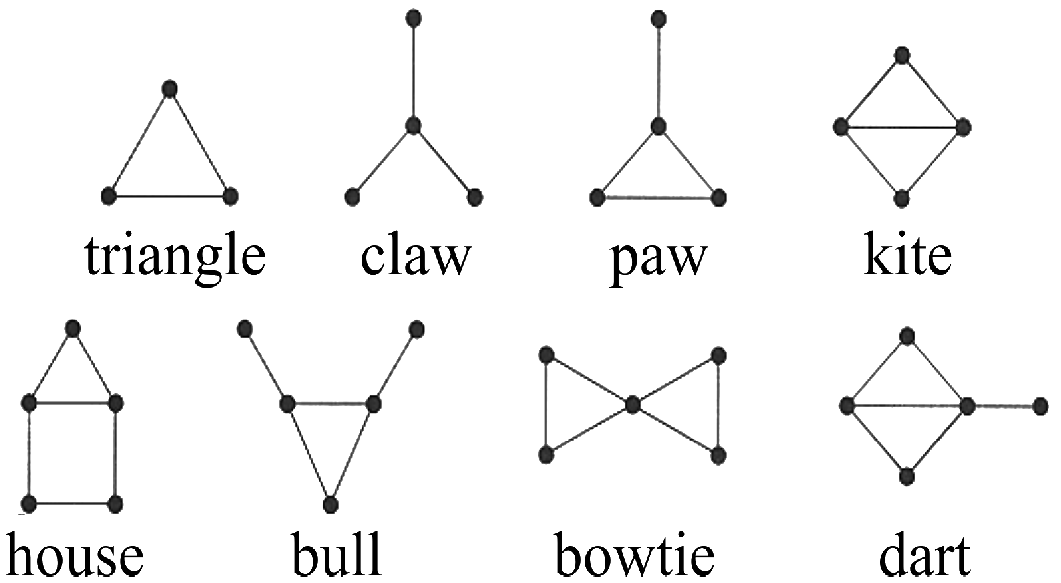
\includegraphics[width=.5\textwidth]{con-graph-menageries}
  \caption{Graph menageries}
  \label{fig:con-graph-menageries}
\end{figure}

\begin{definition}{}{con-petersen}
  (1.1.36. Definition in text)
  A \textbf{Petersen graph} (PG) is the \textbf{simple graph} whose vertices are the 2-element subsets of a 5-element set and whose edges are the pairs of \textbf{disjoint} 2-element subsets.

  The \textbf{girth} of a graph with a cycle is the length of its shortest cycle. A graph with no cycle has infinite girth.
\end{definition}

For a Petersen graph in \cref{def:con-petersen}, in other words, given a simple graph and any 5 elements (like 1--5 or a--e), if there are exactly two different elements (as an unordered set) chosen from the 5 elements on each vertex, and if the endpoints of each edge have distinct numbers, such a graph is a Petersen graph. For example, the leftmost graph in \cref{fig:con-petersen-examples}.

As you can see in the leftmost graph in \cref{fig:con-petersen-examples}, the topmost vertex has elements $\{ 1,\, 2, \}$; its neighbors has $\{ 4,\, 5 \}$, $\{ 3,\, 5 \}$, $\{ 3,\, 4 \}$ respectively. If any two neighbors of the topmost vertex are neighbors (there is a triangle in the graph), you couldn't choose 6 distinct elements out of 5 distinct elements.

For a graph with two cycles: a triangle $C_3$ and a rectangle $C_4$, the girth of that graph is 3, which is the length $C_3$. The minimal possible value of the girth of a graph is 1 in graphs with self-loops. Without a cycle in a graph, the length for a path to go back to the starting vertex without reusing an edge is infinity. That is, impossible.

\begin{figure}[htbp]
  % TODO: TikZ version
  \centering
  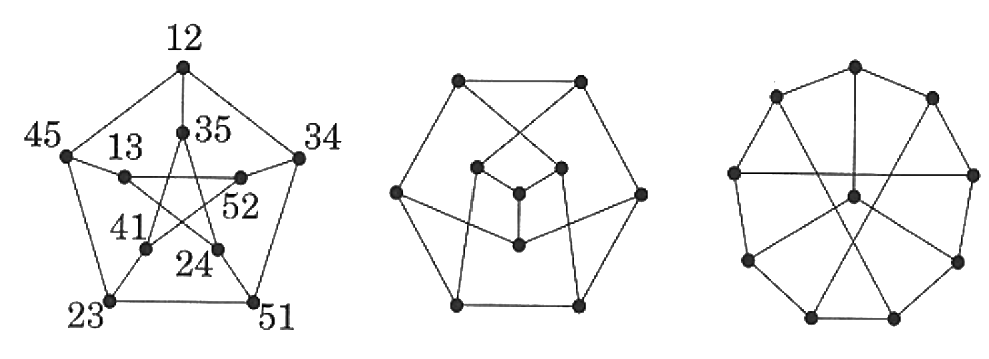
\includegraphics[width=.5\textwidth]{con-petersen-examples}
  \caption{Examples of Petersen graphs.}
  \label{fig:con-petersen-examples}
\end{figure}

\begin{proposition}{}{con-petersen-neighbor}
  (1.1.38. Proposition in text)
  If two vertices are nonadjacent in Petersen graph, then they have exactly one common neighbor.
\end{proposition}

\textbf{Proof} of \cref{prop:con-petersen-neighbor}:

\begin{enumerate*}
  \item Any two nonadjacent vertices share one element, and their union $S$ has 3 elements.
        \begin{enumerate}
          \item For example, the vertices 12 and 23 in the leftmost graph in \cref{fig:con-petersen-examples} share the element 2.
          \item For a simple graph with three vertices and two edges, there are 6 elements chosen from 5 elements for three vertices. As a result, at least one element appears twice in this graph. This is proven by \cref{princ:intro-pigeonhole} (pigeonhole principle).
        \end{enumerate}
  \item A vertex adjacent to two vertices is a 2-set (a set with two elements) disjoint from both its neighbors.
  \item Since the 2-sets are chosen from $\{ 1,\, 2,\, 3,\, 4,\, 5 \}$, there is exactly one 2-set disjoint from $S$ (defined in the first point).
\end{enumerate*}

\begin{corollary}{}{con-petersen-girth}
  (1.1.40. Corollary in text)
  The Petersen graph has girth 5.
\end{corollary}

\textbf{Proof} of \cref{cor:con-petersen-girth}:
\begin{enumerate*}
  \item The graph is simple, for it has no 1-cycle or 2-cycle.
  \item A 3-cycle require three pairwise disjoint 2-sets, which can not occur among 5 elements.
  \item A 4-cycle in the absence of 3-cycles would require nonadjacent vertices with two common neighbors, which violates \cref{prop:con-petersen-neighbor}.
  \item The vertices 12, 34, 51, 23, 45 form a 5-cycle, so the girth is 5.
\end{enumerate*}

In the proof above, it proves \cref{cor:con-petersen-girth} by proving the impossibility of 1-cycle, 2-cycle, 3-cycle and 4-cycles. We don't need to prove cycles with more than 5 vertices because the girth of a graph is defined by the shortest cycle, which is 5 in the Petersen graph.

\subsubsection{Automorphism}

\begin{definition}{}{}
  (1.1.41. Definition in text)
  An \textbf{automorphism} of $G$ is an isomorphism from $G$ to $G$.

  A graph $G$ is \textbf{vertex-transitive} if for every pair $u,\, v \in V(G)$, there is an automorphism that maps $u$ to $v$.
\end{definition}

Automorphism refers to an isomorphism for only one single graph. \supp{By humand eyes, we regard symmetric objects beautiful.} In graph theory, if we make swaps of vertices such that the graph is identical to the original one, we get a automorphism for these swapping.

\begin{wrapfigure}{r}{0.3\textwidth}
  % TODO: TikZ version
  \centering
  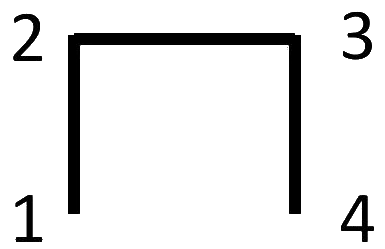
\includegraphics[width=.28\textwidth]{con-automorphism-en}
  \caption{A graph $G$ in N shape.}
  \label{fig:con-automorphism-en}
\end{wrapfigure}

(1.1.42.* Example in text) For example, $G$ as shown in \cref{fig:con-automorphism-en} is the path with $V(G) = \{ 1,\, 2,\, 3,\, 4 \}$ and $E(G) = \{ 12,\, 23,\, 34 \}$. It has two automorphisms: (1) the identity permutation (a vertex swapping with itself) and (2) the permutation $1 \leftrightarrow 4$ and $2 \leftrightarrow 3$ because we could mirror the vertices 1 and 2 to vertices 4 and 3 respectively such that the graph "looks" as the original one without a bijection function.

Question 1: Is it an automorphism if only vertices 1 and 2 are swapped in $G$?\\
Answer: No. Since we need a bijection function to make the swapped graph "look like" the original one, it's not an automorphism; it's an isomorphism.

Question 2: Is $G$ isomorphic to the graph $H$ which is obtained from only swapping vertices 1 and 2 of $G$?\\
Answer: Yes. Please refer to the previous answer.

\begin{wrapfigure}{r}{0.3\textwidth}
  % TODO: TikZ version
  \centering
  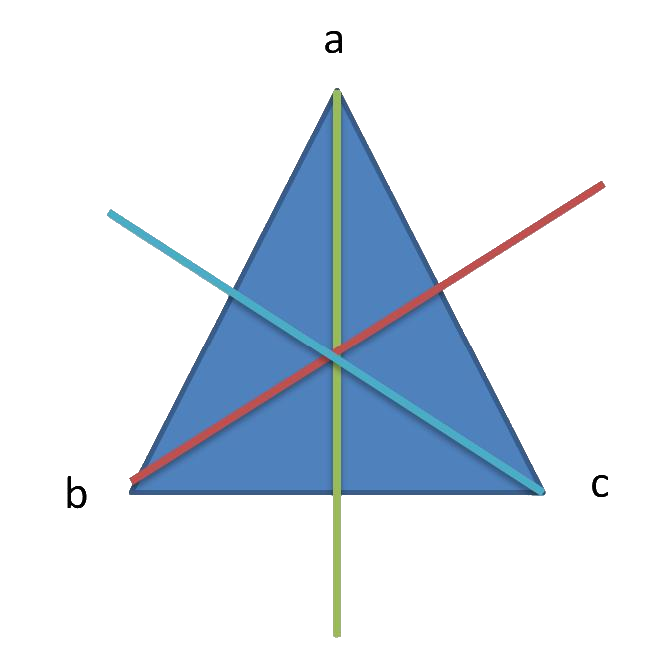
\includegraphics[width=.28\textwidth]{con-automorphism-triangle}
  \caption{A graph $G$ in triangle.}
  \label{fig:con-automorphism-triangle}
\end{wrapfigure}

Given a graph $G$ as shown in \cref{fig:con-automorphism-triangle}, we know that automorphism of $G$ is a permutation function $\func{P}{V(G)}{V(G)}$ such that $P(u)P(v) \in E(G) \iff uv \in E(G)$. That is, the permutation function $P$ preserves adjacency and non-adjacency in graph $G$.

Along the green line passing through the vertex $a$, by mirroring the graph (swapping vertices $b$ and $c$), we have the following mapping of vertices before and after:
\begin{enumerate*}
  \def\mapping#1#2{Old vertex $#1$ $\rightarrow$ new vertex $#2$.}%
  \item \mapping{a}{a}
  \item \mapping{b}{c}
  \item \mapping{c}{b}
\end{enumerate*}

Not only can we mirror a graph, but also we can rotate a graph as follows.

In matrix representation of an automorphism, the first (topmost) row is the vertices before mapping; the last (bottom) row is the mapped ones.

In clause representation (?) of an automorphism, each vertex in a clause (a pair of parentheses) rotates left.

Identity automorphism means vertices are swapped with themselves. Reflection automorphism manes mirroring a graph.

\begin{center}
  % TODO: LaTeX version
  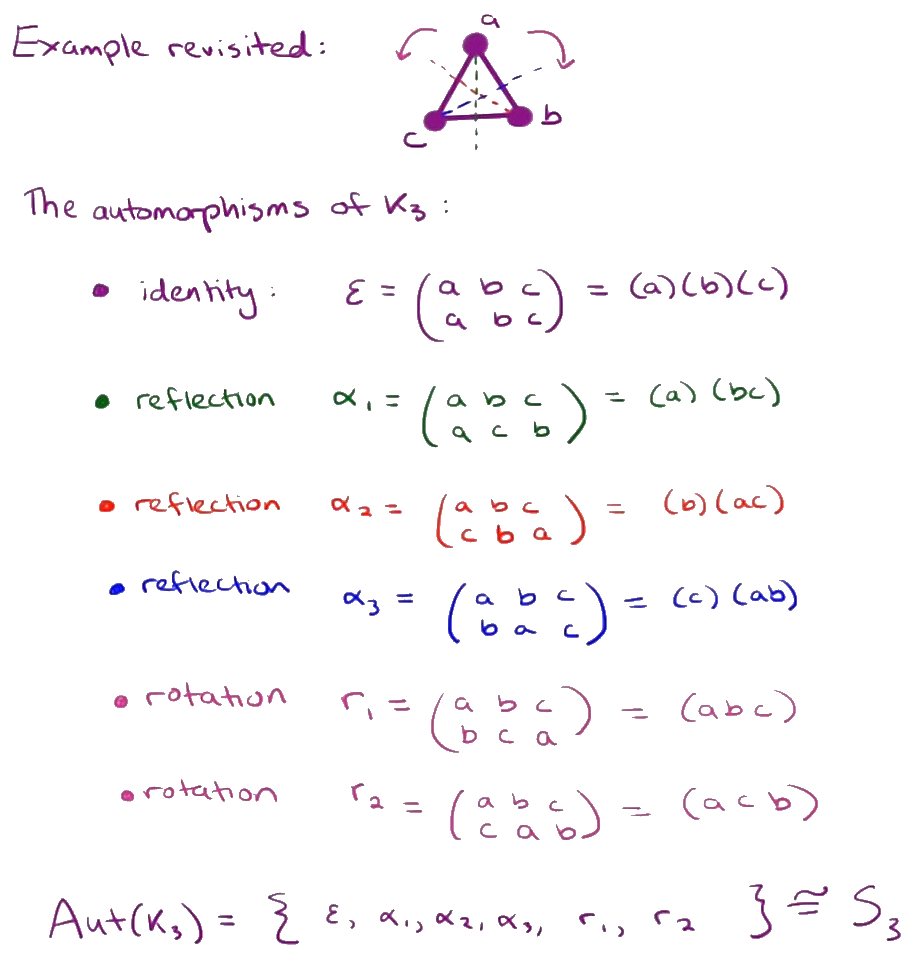
\includegraphics[width=.5\textwidth]{con-automorphism-rotation}
\end{center}

How can you say that a graph is more symmetric than the other one? You need the calculate the number of automorphisms in them.

\begin{center}
  % TODO: LaTeX version
  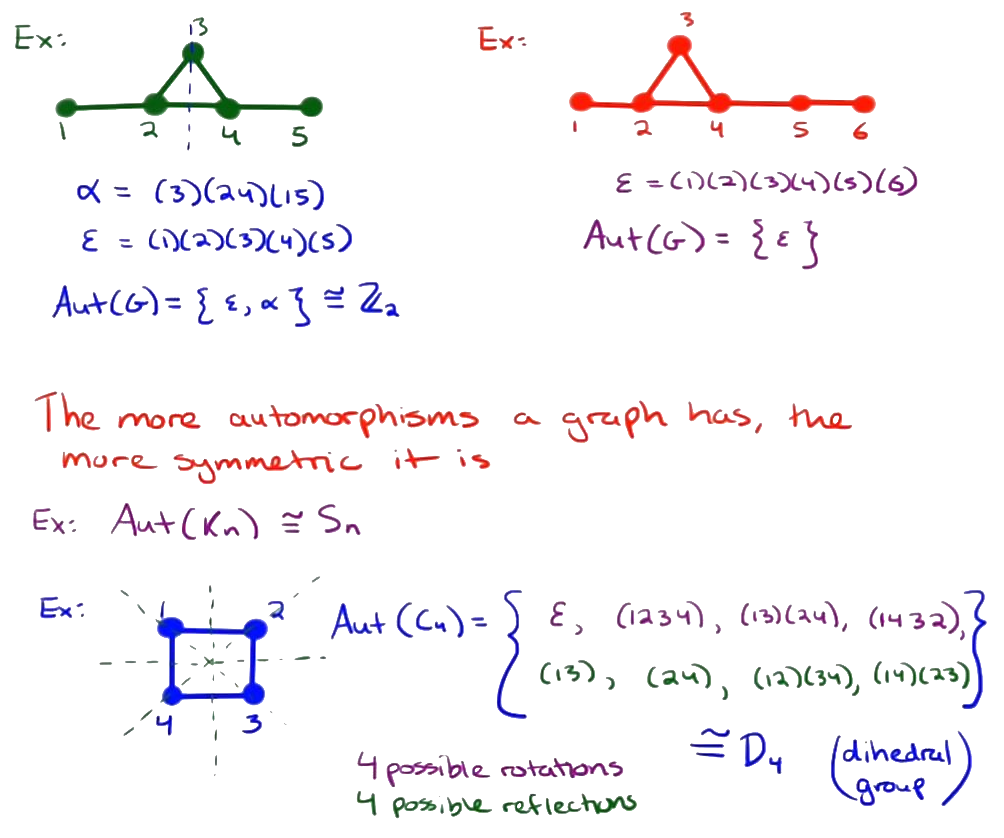
\includegraphics[width=.5\textwidth]{con-automorphism-comparison}
\end{center}
The characteristics of automorphisms are important to some extent.

Reference: Sarada Herke. (2015). "Graph Theory FAQs: 02. Graph Automorphisms" on YouTube. [Online]. \url{https://www.youtube.com/watch?v=X4_4Bqj6EdA}. Accessed on 2024-03-28.

\subsubsection{Paths, Cycles and Trails}

\begin{definition}{}{con-walk-trail}
  (1.2.2. Definition in text)
  A \textbf{walk} is a list $v_0,\, e_1,\, v_1,\, \ldots,\, e_k,\, v_k$ of vertices and edges, such that for $1 \leq i \leq k$, the edges $e_i$ has endpoints $v_{i-1}$ and $v_i$.

  A \textbf{trail} is a walk with \textbf{no repeated edge}.
\end{definition}

In a walk or trail, there could be repeated vertices.

For example, recall the seven bridge problem in \cref{subsubsec:con-seven-bridges}. The list $W_1$ below is a closed walk of length 5 rather than a trail. The list $T_1$ below is a trail.

\begin{align*}
  W_1 = x,\, e_2,\, w,\, e_5,\, y,\, e_6,\, x,\, e_1,\, w,\, e_2,\, x \\
  T_1 = x,\, e_2,\, w,\, e_5,\, y,\, e_6,\, x,\, e_1,\, w
\end{align*}

% TODO FIXME: modify \reusablefigure to receive subfigure
\begin{figure}[ht]
  % TODO: TikZ version
  \centering
  \begin{subfigure}{0.35\textwidth}
    \centering
    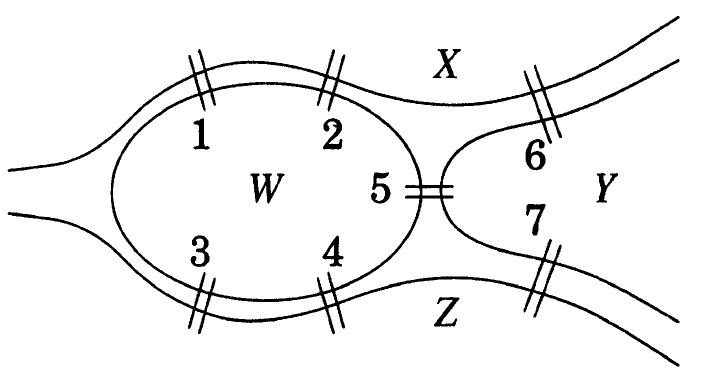
\includegraphics[width=\textwidth]{con-seven-bridge-original}
    \caption{Original version.}
  \end{subfigure}
  \hfil
  \begin{subfigure}{0.25\textwidth}
    \centering
    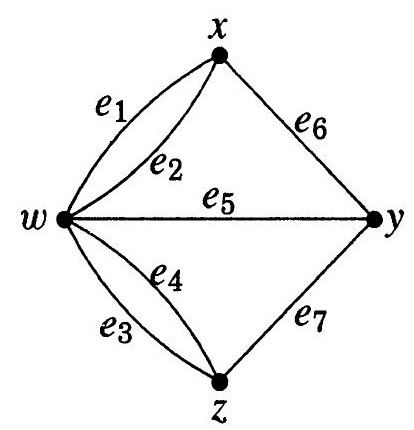
\includegraphics[width=\textwidth]{con-seven-bridge-graph}
    \caption{Graph version.}
  \end{subfigure}
  \caption{Seven-bridge problem.}
\end{figure}

\begin{definition}{}{con-walk-trail-path-endpoints}
  (1.2.2. Definition in text)
  A \textbf{$\bm{u,v}$-walk} or \textbf{$\bm{u,v}$-trail} has first vertex $u$ and last vertex $v$ as its endpoints.
  (A walk or a trail records vertices and edges especially in a multigraph.)

  A \textbf{$\bm{u,v}$-path} is a path whose vertices of degree 1 are $u$ and $v$; the others are \textbf{internal vertices} (usually of degree 2). (A path only records vertices.)

  The \textbf{length} of a walk, trail, path or cycle is the \textbf{number of edges}. (In the length of a path is the number of its vertices minus one.)

  A wal or trail is \textbf{closed} if its endpoints are the same.
\end{definition}

In brief, a $u,v$-path refers to a way to traverse some vertices from $u$ to $v$ via some edges.

See \cref{def:con-path-cycle} for the definition of paths and cycles.

\begin{figure}[htbp]
  % TODO: TikZ version
  \centering
  \begin{subfigure}[t]{.4\textwidth}
    \centering
    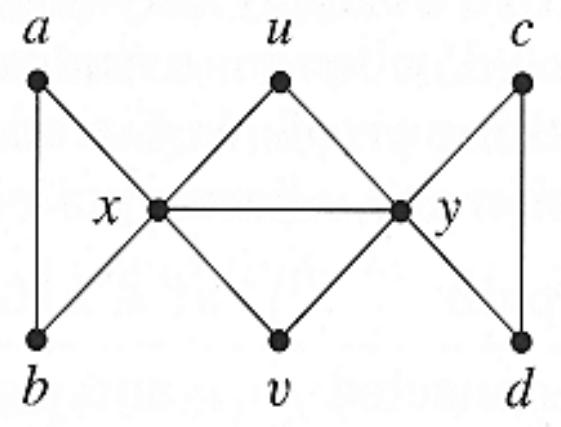
\includegraphics[width=.8\textwidth]{con-walk-original}
    \caption{The original graph with nothing drawn.}
    \label{fig:con-walk-original}
  \end{subfigure}
  \hspace{.1\textwidth}
  \begin{subfigure}[t]{.4\textwidth}
    \centering
    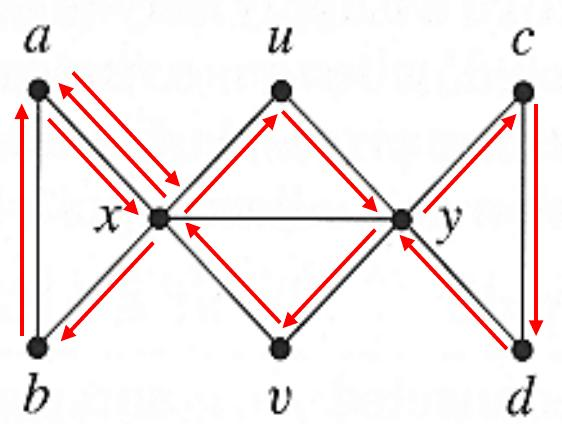
\includegraphics[width=.8\textwidth]{con-walk-closed}
    \caption{A closed $a,a$-walk or an $a,a$-cycle.}
    \label{fig:con-walk-closed}
  \end{subfigure}

  \vspace{2em}

  \begin{subfigure}[t]{.4\textwidth}
    \centering
    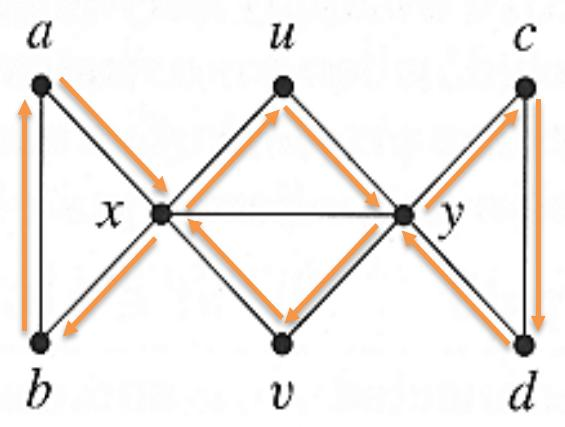
\includegraphics[width=.8\textwidth]{con-trail-closed}
    \caption{A closed $a,a$-trail or an $a,a$-cycle.}
    \label{fig:con-trail-closed}
  \end{subfigure}
  \hspace{.1\textwidth}
  \begin{subfigure}[t]{.4\textwidth}
    \centering
    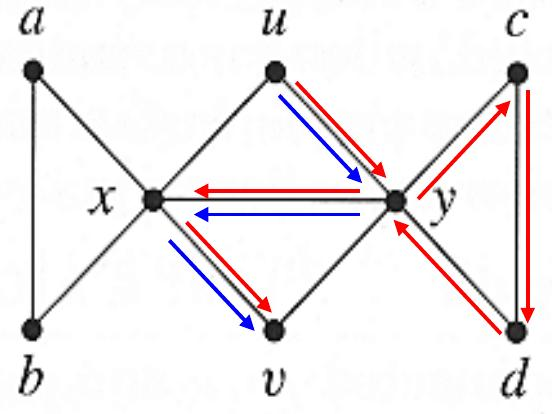
\includegraphics[width=.8\textwidth]{con-trail-path}
    \caption{A $u,v$-trail $u,\, y,\, c,\, d,\, y,\, x,\, v$ contains $u,v$-path $u,\, y,\, x,\, v$ but not $u,\, y,\, v$.}
    \label{fig:con-trail-path}
  \end{subfigure}

  \vspace{2em}

  \begin{subfigure}[t]{.4\textwidth}
    \centering
    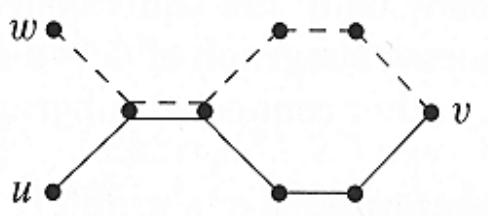
\includegraphics[width=.8\textwidth]{con-walk-path-example}
    \caption{A $u,v$-walk contains a $u,w$-path. See \cref{lem:con-walk-path} and its proof.}
    \label{fig:con-walk-path-example}
  \end{subfigure}
  \hspace{.1\textwidth}
  \begin{subfigure}[t]{.4\textwidth}
    \centering
    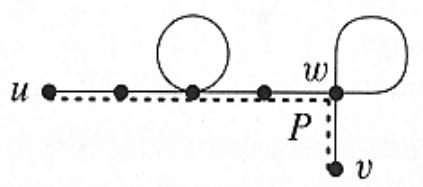
\includegraphics[width=.8\textwidth]{con-walk-path-proof}
    \caption{A graph for the illustration of the proof of \cref{lem:con-walk-path}.}
    \label{fig:con-walk-path-proof}
  \end{subfigure}

  \caption{Illustrations for walks and trails.}
  \label{fig:con-walk-trail}
\end{figure}

\begin{theorem}{String Principle of Induction}{con-strong-induction}
  (1.2.1. Theorem in text)
  Let $P(n)$ be a statement with an integer parameter $n$.
  If the following two conditions hold, then $P(n)$ is true for each positive integer $n$.

  \begin{enumerate*}
    \item P(1) is true.
    \item For all $n > 1$, "$P(k)$ is true for $1 \leq k < n$" implies "$P(n)$ is true".
  \end{enumerate*}
\end{theorem}

Continuing from \cref{thm:con-strong-induction}, if you cannot show that "all" cases from the base case $P(1)$ to $P(n-1)$ true, you cannot use strong principle of induction to say $P(n)$ true.

In strong principle of induction in \cref{thm:con-strong-induction} we prove $P(n)$ true under $P(1)$ to $P(n - 1)$ true, rather than proving $P(n + 1)$ true under $P(1)$ to $P(n)$ true as we do in principle of induction in \cref{princ:intro-induction}.

\begin{lemma}{}{con-walk-path}
  (1.2.5. Lemma in text)
  Every $u,v$-walk contains a $u,v$-path.
\end{lemma}

Note that proof of a theorem (lemma, principle, $\ldots$) must be applicable for all graphs in the domain instead of some limited cases. And you couldn't assume $P(n - 1)$ true without a proof because $P(n - 1)$ may be false.

\textbf{Proof} of \cref{lem:con-walk-path} using strong principle of induction in \cref{thm:con-strong-induction}:
By induction for a $u,v$-walk $W$ whose length is $l$ as illustrated in \cref{fig:con-walk-path-proof}:
\begin{enumerate*}
  \item Basis step: When $l = 0$, $W$ contains a single vertex as a path whose length is 0.
  \item Induction step: When $l \geq 1$, there are two possible cases as follows.
        \begin{enumerate}
          \item Case 1: $W$ has no repeated vertex, so $W$ is a $u,v$-path (if we see only the sequence of vertices in $W$).
          \item Case 2: $W$ has a repeated vertex $w$. (This case covers all cases with any positive number of repeated vertices.) Thus, there is a $u,u$-loop or $u,u$-cycle. By removing that loop or cycle, we get a $u,v$-path.
        \end{enumerate}
\end{enumerate*}

\begin{definition}{}{con-connected-path}
  (1.2.6. Definition in text)
  A graph $G$ is \textbf{connected} if it has a $u,v$-path whenever $u,v \in V(G)$; otherwise, $G$ is \textbf{disconnected}.

  If $G$ has a $u,v$-path, then $u$ is \textbf{connected} to $v$ in $G$.

  The \textbf{connection relation} on $V(G)$ consists of the \textbf{ordered pairs} $(u,\, v)$ such that $u$ is connected to $v$. (In our primary textbook, $uv$ refers to an edge between $u$ and $v$ while $(u,\, v)$ may not imply an edge $uv$; $(u,\, v)$ means that there is an $u,v$-path. Also note that $(u,\, v)$ and $(v,\, u)$ ($u \neq v$) refer to two different paths.)
\end{definition}

Note that the concept of a \textit{connected} graph is defined on vertices instead of edges. If a graph $G$ is connected, all ordered pairs of vertices in the cartesian product (\cref{rem:intro-tuple-ordered-pair}) $V(G) \times V(G)$ have paths.

Connection relation is also an equivalence relation (\cref{def:intro-equiv-relation}), which satisfies reflexive, symmetric, transitive properties:
\begin{enumerate*}
  \item Reflexive property: Any vertex has connection to itself; that is, in a given graph, $(u,\, u)$ is a part of the connection relation for any vertex $u$.
  \item Symmetric property: In an unordered graph, "$u$ is connected to $v$" implies "$v$ is connected to $u$".
  \item Transitive property: $(v_1,\, v_2)$ and $(v_2,\, v_3)$ imply $(v_1,\, v_3)$.
\end{enumerate*}

\begin{example}{}{con-connected-graph}
  \begin{wrapfigure}{r}{.3\textwidth}
    % TODO: TikZ version
    \centering
    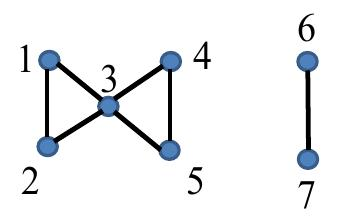
\includegraphics[width=.28\textwidth]{con-connected-path}
    \caption{A graph $G$ to illustrate connection relation.}
    \label{fig:con-connected-path}
  \end{wrapfigure}

  \textbf{Question 1}: Is the graph $G$ in \cref{fig:con-connected-path} connected? List all equivalence classes.

  \textbf{Answer}: There are two equivalence classes, $\{1,\, 2,\, 3,\, 4,\, 5\}$ and $\{6,\, 7\}$, so this graph is not connected. These two equivalence classes form two connected components (maximal connected subgraphs; \cref{def:con-component}).

  \textbf{Question 2}: How to write the connection relation on $V(G)$ in \cref{fig:con-connected-path}?

  \textbf{Answer}: $\{ 1,\, 2,\, 3,\, 4,\, 5 \}^2, \{ 6,\, 7 \}^2$. (Please refer to the cartesian product defined in \cref{rem:intro-tuple-ordered-pair}.)
\end{example}

\begin{remark}{}{con-maximum}
  \textbf{Minimal}/\textbf{maximal} somethings are conditional or local minimums/maximums, while \textbf{minimum}/\textbf{maximum} is globally minimum/maximum without conditions.

  E.g., I have the \textbf{maximal} height among people \textit{under 155cm} in this classroom. Amy has the \textbf{maximal} height among people around her.
\end{remark}

\begin{definition}{}{con-component}
  (1.2.8. Definition in text)
  The \textbf{connected components} or \textbf{components} of a graph $G$ are its (locally) \textbf{maximal} connected subgraphs.

  \textbf{A maximal connected subgraph of $\bm{G}$ is a subgraph that is connected and is not contained in any other subgraph.}

  A component is \textbf{trivial} if it has no edges; that is, it is a vertex.

  An \textbf{isolated vertex} is a vertex of degree 0.
\end{definition}

\begin{figure}[htbp]
  % TODO: TikZ version
  \centering
  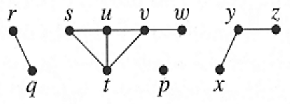
\includegraphics[width=.3\textwidth]{con-connected-components}
  \caption{There are 4 components in this graph, where the isolated vertex $p$ forms a trivial component $\{p\}$.}
  \label{fig:con-component}
\end{figure}

For \cref{def:con-component}, a graph may have multiple maximal connected subgraphs. A connected subgraph may not be maximal, saying vertices 1, 2 and 3 in \cref{fig:con-connected-path}. If we couldn't find a vertex to make a component larger while making it connected, such a component is a maximal connected subgraph.

\begin{proposition}{}{con-component}
  Every graph with $n$ vertices and $k$ edges has \textbf{at least} $n - k$ components.
\end{proposition}

Since we are proving \textbf{at least} some values, we could prove that it cannot be less than some values. \supp{It's like when your mother gives you 10 dollars in the morning under the constraint that you need to give back \textbf{at least} 1 dollars at night. It means you can spend \textbf{at most} 9 dollars today; you can spend only 8 dollars though.}

\textbf{Proof} of \cref{prop:con-component}:
\begin{enumerate*}
  \item An $n$-vertex graph with no edges has $n$ components, as shown in the left figure in \cref{fig:con-component-proposition}.
  \item Adding each edge \textbf{decreases} the number of components by \textbf{at least} one ($\leq 1$). From the middle figure to the left figure, the number of component doesn't decrease.
  \item Adding $k$ edges results in the number of components $\geq n - k$. Decreasing at most $k$ components from $n$ components is equivalent to making the number of components $\geq n - k$.
  \item Note that without specifying "at most" or "at least", you may not get full marks in exams.
\end{enumerate*}

\begin{figure}[htbp]
  % TODO: TikZ version
  \centering
  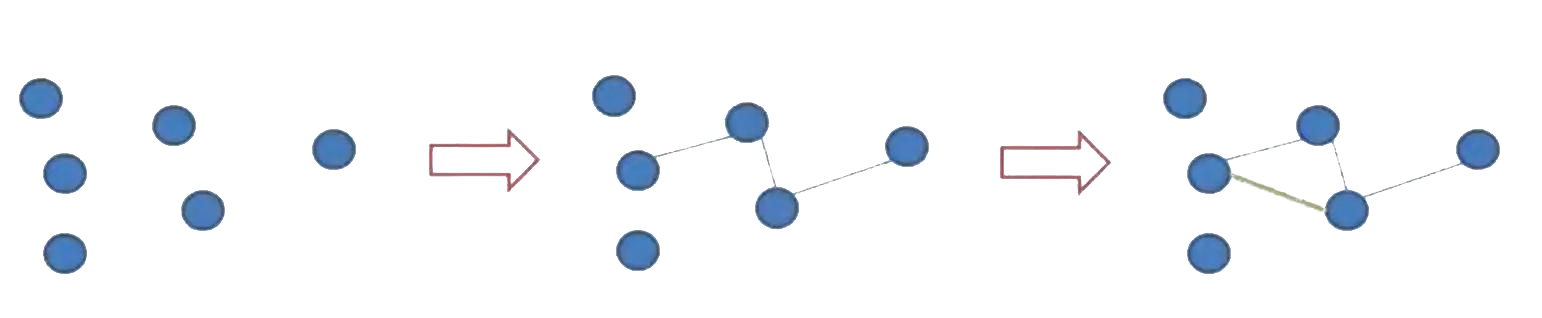
\includegraphics[width=.6\textwidth]{con-component-proposition}
  \caption{An illustration for the proof of \cref{prop:con-component}.}
  \label{fig:con-component-proposition}
\end{figure}

\Cref{prop:con-component} yields that to have a connected graph with $n$ vertices (there is only a component; solve $k$ in $n - k = 1$), you need \textbf{at least} $n - 1$ edges. A \textbf{tree} is a commonly seen connected graph with $n$ vertices and $n - 1$ edges.

\begin{definition}{}{con-cut-edge-vertex}
  A \textbf{cut-edge} or \textbf{cut-vertex} of a graph is an edge or vertex whose deletion increases the number of components.

  Deleting an edge $e$ from $G$ is denoted by $G - e$.
  Similarly, we have $G - v$ for a vertex $v$ in $G$.

  Deleting a set of edges $M$ from $G$ is denoted by $G - M$.
  Similarly, we have $G - S$ for $S$ as a set of vertices of $G$.
\end{definition}

\begin{figure}[htbp]
  % TODO: TikZ version
  \centering
  \begin{subfigure}[t]{.3\textwidth}
    \centering
    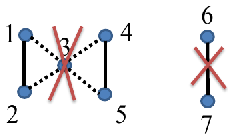
\includegraphics[width=\textwidth]{con-cut-edge}
    \caption{Vertex 3 is a cut-vertex; edge 67 is a cut-edge.}
    \label{fig:con-cut-edge}
  \end{subfigure}
  \hspace{.2\textwidth}
  \begin{subfigure}[t]{.4\textwidth}
    \centering
    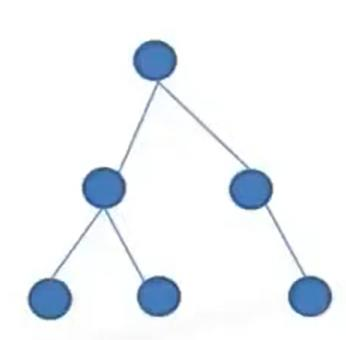
\includegraphics[width=.5\textwidth]{con-cut-edge-tree}
    \caption{In a tree, every edge is a cut-edge. Every non-leaf node (every internal node or the root) is a cut-vertex.}
    \label{fig:con-cut-edge-tree}
  \end{subfigure}
\end{figure}

\begin{definition}{}{con-induced-subgraph}
  When $T \subseteq V(G)$, the \textbf{induced subgraph} $G[T]$ consists of $T$ and all edges whose endpoints are contained in $T$. (induced by vertices)
\end{definition}

\begin{figure}
  % TODO: TikZ version
  \centering
  \begin{subfigure}[t]{.25\textwidth}
    \centering
    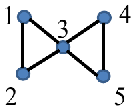
\includegraphics[width=.75\textwidth]{con-induced-subgraph-original}
    \caption{The original graph $G$ whose vertex set is $V(G)$.}
    \label{fig:con-induced-subgraph-original}
  \end{subfigure}
  \hspace{.1\textwidth}
  \begin{subfigure}[t]{.25\textwidth}
    \centering
    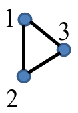
\includegraphics[width=.5\textwidth]{con-induced-subgraph-induced}
    \caption{The induced subgraph $G[T]$, where $T \subseteq V(G)$.}
    \label{fig:con-induced-subgraph-induced}
  \end{subfigure}
  \hspace{.1\textwidth}
  \begin{subfigure}[t]{.25\textwidth}
    \centering
    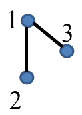
\includegraphics[width=.5\textwidth]{con-induced-subgraph-subgraph}
    \caption{A subgraph of $G$ but not an induced subgraph of $G$ because it lacks edge 23 which is in $G$.}
    \label{fig:con-induced-subgraph-subgraph}
  \end{subfigure}
  \caption{An example for induced subgraphs.}
  \label{fig:con-induced-subgraph}
\end{figure}

For \cref{def:con-induced-subgraph}, note that:
\begin{enumerate*}
  \item $T$ is a subset of vertices.
  \item $E_T = \left\{ uv \in E(G): u \in T,\, v \in T \right\}$. That is, after we choose some vertices $T$ from the graph $G$, all edges related to vertices $T$ are preserved, and there is no additional edge.
  \item $G[T] = (T,\, E_T)$
\end{enumerate*}

\begin{remark}{Biconditional statements}{con-iff}
  The biconditional statement "$P \iff Q$" has the as "$(P \implies Q) \land (Q \implies P)$. We read it as "$P$ if and only if $Q$", where "$Q \implies P$" is "$P$ if $Q$", and "$P \implies Q$" is "$P$ only if $Q$".

  \begin{center}
    \begin{tabular}{ccc}
      \hline
                            & A                        & B                        \\ \hline
      Direct Method         & $P \implies Q$           & $P \implies Q$           \\
      Contrapositive Method & $\neg Q \implies \neg P$ & $\neg P \implies \neg Q$ \\
      Contradiction Method  & $\neg (P \land \neg Q)$  & $\neg (Q \land \neg P)$  \\
      \hline
    \end{tabular}
  \end{center}

  $\neg (P \land \neg Q)$ means that it is impossible for $Q$ false given $P$ true.

  All three statements on the left (column A) are equivalent to one another; same for the right (column B). However, the left column is not equivalent to the right column.

  By rewriting the statement, we could prove the biconditional statement easier (in other words) because $P$ or $Q$ may be hard to be true.
  Instead of using the direct method, we could choose one statement from the left and right columns respectively to prove biconditional statements.
  But practically, it is easier to rewrite the problem to prove it with the other method without crossing methods.
\end{remark}

\begin{theorem}{}{con-cut-edge-cycle}
  P: \underline{An edge is a cut-edge} if and only if Q: \underline{it belongs to no cycle}.
\end{theorem}

\textbf{Proof} of \cref{thm:con-cut-edge-cycle}:
\begin{enumerate}
  \item Instead of using the direct method (proving both $P \implies Q$ and $Q \implies P$), we can use the contrapositive method to prove it.
  \item Let $e = xy$ be an edge, and let $H$ be the component containing $e$.
  \item We want to prove $\neg P$: \underline{$H-e$ is connected} iff. $\neg Q$: \underline{$e$ belongs to a cycle}. $\neg P$ means the graph is still connected after we remove an edge $e$ from $H$, so $e$ is not an cut-edge.
  \item To prove $\neg P \implies \neg Q$, suppose that $H-e$ is connected. Then, $H-e$ contains an $x,y$-path $P(x,\, y)$. $P(x,\, y) + e$ is a cycle of $G$.
  \item To prove $\neg Q \implies \neg P$, let $P$ be a $u,v$-path, given $e$ is on a cycle $C$.
        \begin{enumerate}
          \item If $P$ doesn't contain the edge $e$, removing the edge $e$ doesn't affect $P$, and the graph $H$ is still connected.
          \item If $P$ contains the edge $e$, since $e$ is on a cycle, there can still be a $u,v$-path but not through the edge $e$, making the graph $H-e$ connected. See \cref{fig:con-cut-edge-cycle} for the illustration.
        \end{enumerate}
\end{enumerate}

\begin{figure}[htbp]
  % TODO: TikZ version
  \centering
  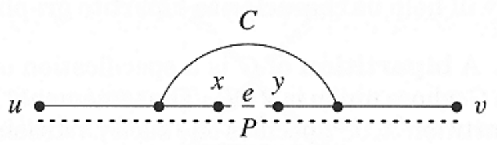
\includegraphics[width=.28\textwidth]{con-cut-edge-cycle}
  \caption{The illustration of $e$ on a cycle $C$ and on a $u,v$-path.}
  \label{fig:con-cut-edge-cycle}
\end{figure}

\begin{lemma}{}{con-walk-cycle}
  Every closed odd walk contains an odd cycle.
\end{lemma}

\textbf{Proof} of \cref{lem:con-walk-cycle}: By induction on length $l$ of a closed walk $W$.
\begin{enumerate*}
  \item Basis step: $l = 1$, which means a self-loop.
  \item Suppose that a closed odd walk whose length $l$ satisfies $1 \leq l < W$. Note that the walk is both closed and odd in \cref{lem:con-walk-cycle}; you cannot apply mathematical induction on a wrong foundation.
  \item Induction step: $l > 1$:
        \begin{enumerate}
          \item Case 1: $W$ has no repeated vertex other than the first and last vertices being the same. So, $W$ itself forms a desired cycle.
          \item Case 2: $W$ contains a repeated vertex $v$. Saying vertex $v$ in the walk in \cref{fig:con-walk-cycle}, for some repeated vertex $v$, such a vertex partitions the walk into two cycles, where one is odd length and the other is even length, so we have an odd cycle in an odd walk.
        \end{enumerate}
  \item As shown in \cref{fig:con-walk-cycle}, for a $v-v$-cycle for vertices on the left of $v$, there is a 5-cycle. However, for the cycle on the right, closed even walks are not covered by \cref{lem:con-walk-cycle}. The base is important.
\end{enumerate*}

\begin{figure}
  % TODO: TikZ version
  \centering
  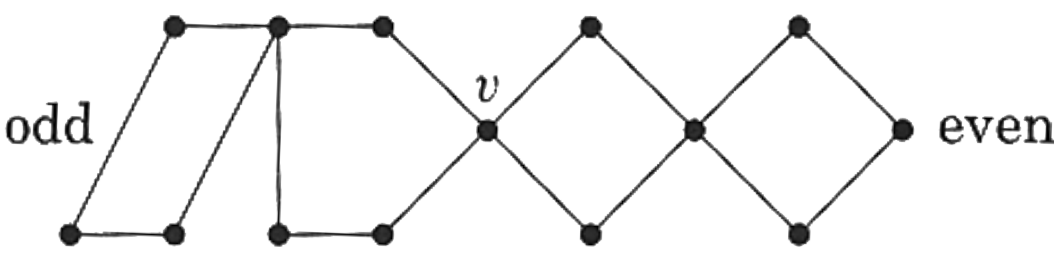
\includegraphics[width=.5\textwidth]{con-walk-cycle}
  \caption{An illustration for \cref{lem:con-walk-cycle}.}
  \label{fig:con-walk-cycle}
\end{figure}

\begin{definition}{}{con-bipartition}
  A \textbf{bipartition} of $G$ is a specification of two disjoint independent sets in $G$ whose union is $V(G)$. Note two \textit{disjoint} sets refers to two sets without a vertex in both sets; an independent set refers to a set without an edge within.

  An \textbf{$\bm{X,Y}$-bigraph} is \textbf{a} bipartite graph with bipartition $X$ and $Y$.
\end{definition}

Recall \cref{def:con-bipartite} as follows.
\recall{con-bipartite}
\begin{figure}[htbp]
  \centering
  \bipartitegraphwithlabels
\end{figure}

In an independent set, there is no edge (\cref{def:con-complement}). If two sets are disjoint, they share no vertex (\cref{def:intro-set-operations}). They refer to different characteristics.

\begin{theorem}{}{con-bipartite-odd-cycle}
  A graph is bipartite iff. it has no odd cycle.
\end{theorem}

\textbf{Proof} of \cref{thm:con-bipartite-odd-cycle}:

$\Rightarrow$: In each of the two partite sets, since there is no edge, there cannot form a cycle. So, every walk alternates between two partite sets. Thus, return to return to the original partite set, it requires an even number of edges, and form no odd cycle.

$\Leftarrow$: In this direction, we use the direct method to prove it.

Case 1 for $\Leftarrow$:
\begin{enumerate}
  \item Let $G$ be a graph with no cycle. Without a cycle in $G$, there is no odd cycle.
  \item Case a: If $G$ has no edges, we can partition vertices into two sets and get a bipartite graph.
  \item Case b: If $G$ has edges (has only vertices), by putting the endpoints of each edges into two different sets, we get two disjoint independent sets. For zero-degree vertices, they can be in one of the two disjoint sets with the graph remaining bipartite.
\end{enumerate}

Case 2 for $\Leftarrow$:
\begin{enumerate}
  \item With cycles but without an odd cycle in graph $G$, to prove $G$ bipartite, we need to find the specification of bipartition. That is, we want to find two disjoint independent sets in $G$.
  \item Suppose in $G$ there is a connected component (CC) denoted by $H$, which includes vertices $a$, $b$ and $v$.
  \item Let $f_v(x)$ be a function to calculate the minimum distance from vertex $x$ to $v$ for any vertex $x \in H$. $f_v(v) = 0$. This function is the key point in this proof to partition vertices into two disjoint sets.
  \item For any vertex $u \in H$, $f_v(x)$ is either odd or even.
  \item Put vertices with odd $f_v(x)$ to a set, an even to the other set, as the disjoint sets $X$ and $Y$ illustrated in \cref{fig:con-bipartite-odd-cycle}. $X = \left\{x \in V(H): f_v(x) \text{ is even} \right\}$ and $Y = \left\{y \in V(H): f_v(y) \text{ is odd} \right\}$.
  \item Case a:
        \begin{enumerate}
          \item For any vertices $a$ and $b$ with odd $f_v(x)$ (in the set $X$), by having an $ab$ edge, we get a closed odd walk because $\text{odd} + \text{odd} + 1 = \text{odd}$, as illustrated in \cref{fig:con-bipartite-odd-cycle-odd}.
          \item By \cref{lem:con-walk-cycle}, this closed odd walk contains an odd cycle, and it contradicts to the assumption of case 2 (no odd cycle). As a result, there is no edge in the set $X$ (odd $f_v(x)$ vertices), so the set $X$ is independent.
        \end{enumerate}

  \item Case b:
        \begin{enumerate}
          \item For any vertices $a$ and $b$ with even $f_v(x)$ (in the set $Y$), since $f_v(x)$ is even, there is no $va$ or $vb$ edge to make $f_v(x)$ odd.
          \item By having an $ab$ edge, we get a closed odd walk, as illustrated in \cref{fig:con-bipartite-odd-cycle-even}. By \cref{lem:con-walk-cycle}, this closed odd walk contains an odd cycle, and it contradicts to the assumption of case 2. As a result, there is no edge in the set $Y$ (even $f_v(x)$ vertices), so the set $Y$ is independent.
        \end{enumerate}

  \item By cases a and b, we prove that any component $H \in G$ is an $X,Y$-bigraph. By iterating through all components, we can find bipartition $X$ and $Y$ for $G$ to prove $G$ bipartite.
\end{enumerate}

\begin{figure}[htbp]
  % TODO: TikZ version
  \centering
  \begin{subfigure}[t]{.3\textwidth}
    \centering
    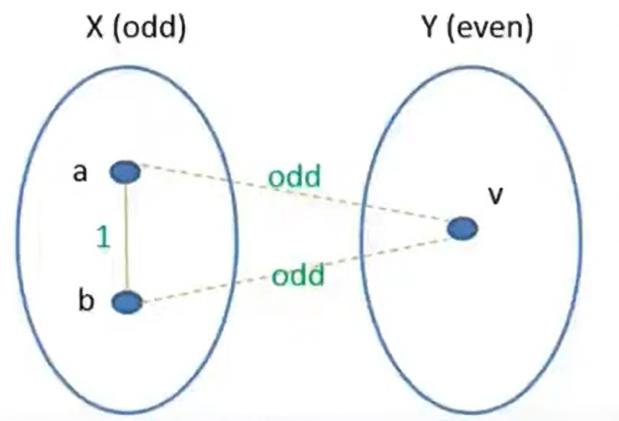
\includegraphics[width=\textwidth]{con-bipartite-odd-cycle-odd}
    \caption{Case 2a}
    \label{fig:con-bipartite-odd-cycle-odd}
  \end{subfigure}
  \hspace{.2\textwidth}
  \begin{subfigure}[t]{.3\textwidth}
    \centering
    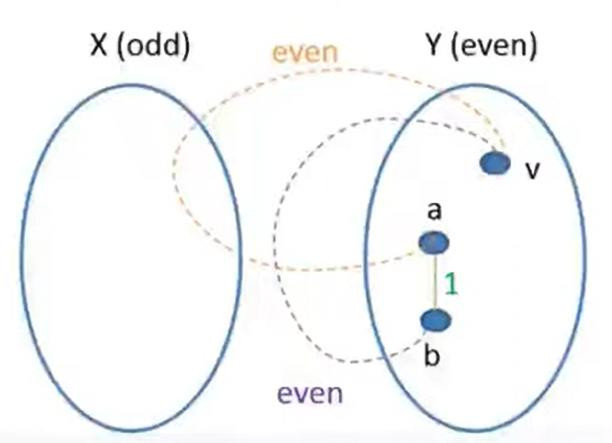
\includegraphics[width=\textwidth]{con-bipartite-odd-cycle-even}
    \caption{Case 2b}
    \label{fig:con-bipartite-odd-cycle-even}
  \end{subfigure}
  \caption{The graphs to illustrate the proof of \cref{thm:con-bipartite-odd-cycle}.}
  \label{fig:con-bipartite-odd-cycle}
\end{figure}

Eulerian solved the seven-bridge problem (\cref{subsubsec:con-seven-bridges}), and define Eulerian graphs related to the seven-bridge problem.

\begin{definition}{}{con-eulerian}
  A graph is \textbf{Eulerian} if it has a \underline{closed trail containing all edges}.

  Recall \cref{def:con-walk-trail}: A trail is a walk with \underline{no repeated edge}. (vertex can be repeated)

  A \textbf{circuit} is a \ul{closed trail} when we do \ul{not specify the first vertex} but \ul{keep the list in cyclic order}.

  An \textbf{Eulerian circuit} or \textbf{Eulerian trail} in a graph is a circuit or trail containing all the edges.
\end{definition}

\begin{lemma}{}{con-degree-cycle}
  If every vertex $v$ of a graph $G$ has degree at least 2, then $G$ contains a cycle.
\end{lemma}

\textbf{Proof} of \cref{lem:con-degree-cycle}:
\begin{enumerate}
  \item Let $P$ be a \underline{maximal} path (\cref{rem:con-maximum}) from a given $v$ in a graph $G$ in which every vertex has degree at least 2 as illustrated in \cref{fig:con-degree-cycle}. Say that the other endpoint of $P$ is $u$.
  \item Since the vertex $u$ is at least degree 2, there must be a edge from $u$ to some vertex in $P$, and it forms a cycle. Otherwise, $P$ is not a maximal path.
  \item Note: A path usually has no repeated vertex.
\end{enumerate}

\begin{figure}[htbp]
  % TODO: TikZ version
  \centering
  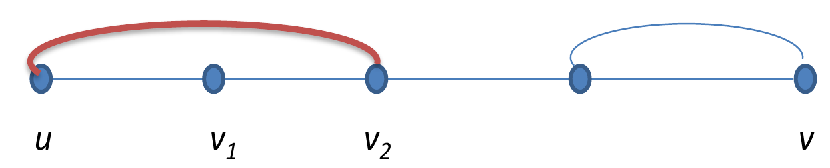
\includegraphics[width=.3\textwidth]{con-degree-cycle}
  \caption{A graph to illustrate the proof of \cref{lem:con-degree-cycle}.}
  \label{fig:con-degree-cycle}
\end{figure}

\begin{theorem}{}{con-eulerian-component-degree}
  A graph $G$ is Eulerian if and only if \ul{it has \textbf{at most} one nontrivial component} and \ul{all its vertices have \textbf{even degree}}.
\end{theorem}

Recall \cref{def:con-component}. A trivial component is a component with only a vertex.

For a graph with only a vertex without edges, since it doesn't violate \cref{thm:con-eulerian-component-degree}, such a graph is Eulerian. This is a special case not covered in the proof above.

\textbf{Proof} of \cref{thm:con-eulerian-component-degree}:

$\Rightarrow$: Given that a graph $G$ is Eulerian, let $C$ be an Eulerian circuit of $G$.
\begin{enumerate}
  \item Part a: There cannot be 2 or more (included) nontrivial components. Otherwise, such a graph is disconnected and is not Eulerian.
  \item Part b: Each passage of $C$ through a vertex uses two incident (connected) edges (\cref{def:con-adj}), and the first edge is paired with the last one at the first vertex. It implies that all vertices of the only one nontrivial component are even degree.
\end{enumerate}

$\Leftarrow$: Let assumption of \underline{at most one nontrivial component and its vertices all have even degree} exist.
\begin{enumerate}
  \item We want to prove by induction on the number of edges $m$.
  \item Basis: $m = 0$. $G$ contains only one vertex. (It doesn't violate the definition of a Eulerian graph.)
  \item Induction: $m>0$. (In fact, by assumption, $m$ should be $\geq 2$.)
        \begin{enumerate}
          \item By \cref{lem:con-degree-cycle}, the only one nontrivial component has a cycle $C$.
          \item Let $G' = G - E(C)$. That is, remove all the edges of cycle $C$. Note that $G'$ is an even graph as $C$ has 2 edges at each vertex.
          \item By induction hypothesis, each component of $G'$ has an Eulerian circuit. Merge these circuits along $C$ to obtain an Eulerian circuit of $G$.
          \item See \cref{fig:con-eulerian-component-degree} for an example to illustrate this step.
        \end{enumerate}
\end{enumerate}

\begin{figure}[htbp]
  % TODO: TikZ version
  \centering
  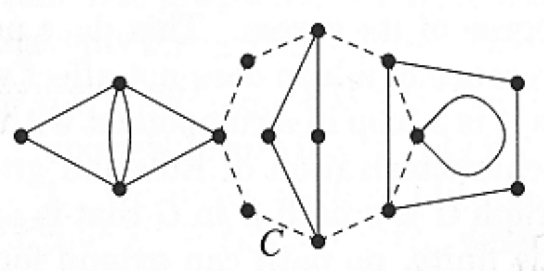
\includegraphics[width=.3\textwidth]{con-eulerian-component-degree}
  \caption{A graph to illustrate the induction step in the right-to-left proof of \cref{thm:con-eulerian-component-degree}.}
  \label{fig:con-eulerian-component-degree}
\end{figure}

\begin{theorem}{}{con-trail-decompose}
  For a connected nontrivial graph with exactly $2 k$ \underline{odd} vertices, the minimum number of trails that decompose it is $\max \{k,\, 1\}$ (the maximum between $k$ and 1).
\end{theorem}

A odd vertex is an odd-degree vertex. A trail is a walk with no repeated vertex. If $k = 0$, it means a graph has only even vertices, and such a graph is Eulerian. $2 k$ odd vertices means the number of odd vertices is even.

Recall \cref{def:con-self-comp}: A \textbf{decomposition} of a graph is a list of subgraphs such that each edge appears in exactly one subgraph in ths list.

\textbf{Proof} of \cref{thm:con-trail-decompose} for a given graph $G$:
\begin{enumerate}
  \item A closed trail contributes even degree to every vertex.\\
        $\Rightarrow$ Each odd vertex has some non-closed trail ending at it.\\
        $\Rightarrow$ $G$ contains at least $k$ trails. (Note that $G$ is Eulerian when $k = 0$.)
  \item Pair up the odd vertices and form $G'$ by adding an "dashed" edge for each pair as shown in \cref{fig:con-trail-decompose-odd-vertices} for 4 odd vertices and $k = 2$ dashed edges.\\
        $\Rightarrow$ $G'$ has an Eulerian circuit $C$.\\
        $\Rightarrow$ By traversing $C$ and starting a new trail when encountering a dashed edge (among $G' - E(G)$), we obtain $k$ trails to decompose $G$. For example, two trails as shown in \cref{fig:con-trail-decompose-decomposition}.
\end{enumerate}

\begin{figure}[htbp]
  % TODO: TikZ version
  \centering
  \begin{subfigure}[t]{.45\textwidth}
    \centering
    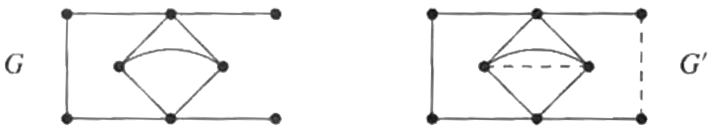
\includegraphics[width=\textwidth]{con-trail-decompose-odd-vertices}
    \caption{Adding "dashed" edges to each pair of odd vertices to form $G'$ from $G$.}
    \label{fig:con-trail-decompose-odd-vertices}
  \end{subfigure}
  \hfill
  \begin{subfigure}[t]{.45\textwidth}
    \centering
    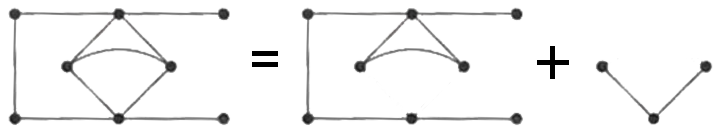
\includegraphics[width=\textwidth]{con-trail-decompose-decomposition}
    \caption{A decomposition of $G$ as two trails.}
    \label{fig:con-trail-decompose-decomposition}
  \end{subfigure}
  \caption{An illustration for the proof of \cref{thm:con-trail-decompose}.}
\end{figure}

\subsection{Vertex Degrees and Counting}

\begin{definition}{}{con-degree}
  The \textbf{degree} of a vertex $v$ in a graph $G$, denoted by $d_G(v)$ or $d(v)$, is the number of edges incident to $v$. Note that each loop at $v$ counts twice (degree 2).

  The \textbf{maximum degree} is $\Delta(G) = \max _{v \in V(G)} \left\{ d_G(v) \right\}$

  The \textbf{minimum degree} is $\delta(G) = \min _{v \in V(G)} \left\{ d_G(v) \right\}$

  $G$ is a \textbf{regular graph} if $\Delta(G) = \delta(G)$. $k$-regular is a graph whose the common degree is $k$. ($\Delta(G) = \delta(G) = k$)

  The \textbf{neighborhood} of $v$, written $N_G(v)$ or $N(v)$, is the set of \ul{vertices} adjacent to $v$.
\end{definition}

\begin{definition}{}{con-order-size}
  The \textbf{order} of a graph $G$, denoted by $n(G)$ or $\abs{V(G)}$, is the number of vertices of $G$.

  The \textbf{size} of a graph $G$, denoted by $e(G)$ or $\abs{E(G)}$, is the number of edges in $G$.
\end{definition}

\subsubsection{Counting and Bijections}

\begin{proposition}{Degree-sum formula}{con-degree-sum}
  If $G$ is a graph, then $\sum_{v \in V(G)} d(v) = 2 e(G)$.
\end{proposition}

\begin{corollary}{}{con-average-degree}
  In a graph $G$, the average vertex degree is $\frac{2 e(G)}{n(G)}$, and hence $\delta(G) \leq \frac{2 e(G)}{n(G)} \leq \Delta(G)$.
\end{corollary}

\begin{corollary}{}{con-odd-degree}
  Every graph has an even number of vertices of odd degree. (The number of odd vertices is even in every graph.)
  
  No graph of odd order is regular with odd degree.
\end{corollary}

\textbf{Proof} of the first sentence in \cref{cor:con-odd-degree}: If there is odd number of odd vertices, $\sum _{v \in V(G)} d(v)$ is odd. It contradicts to \cref{prop:con-degree-sum}. As a result, the number of odd vertices must be even in an undirected graph.

\begin{corollary}{}{con-regular-graph}
  A $k$-regular graph with $n$ vertices has $\frac{n k}{2}$ edges.
\end{corollary}

\subsection{Directed Graphs}

\end{document}